\documentclass{article}

% if you need to pass options to natbib, use, e.g.:
%     \PassOptionsToPackage{numbers, compress}{natbib}
% before loading neurips_2026

% The authors should use one of these tracks.
% Before accepting by the NeurIPS conference, select one of the options below.
% 0. "default" for submission
\usepackage{neurips_2026}
% the "default" option is equal to the "main" option, which is used for the Main Track with double-blind reviewing.
% 1. "main" option is used for the Main Track
%  \usepackage[main]{neurips_2026}
% 2. "position" option is used for the Position Paper Track
%  \usepackage[position]{neurips_2026}
% 3. "eandd" option is used for the Evaluations & Datasets Track
 % \usepackage[eandd]{neurips_2026}
 % if you want to opt-in for a de-anomymized submission (not recommended, but OK):
 %\usepackage[eandd, nonanonymous]{neurips_2026}
% 4. "creativeai" option is used for the Creative AI Track
%  \usepackage[creativeai]{neurips_2026}
% 5. "sglblindworkshop" option is used for the Workshop with single-blind reviewing
 % \usepackage[sglblindworkshop]{neurips_2026}
% 6. "dblblindworkshop" option is used for the Workshop with double-blind reviewing
%  \usepackage[dblblindworkshop]{neurips_2026}

% After being accepted, the authors should add "final" behind the track to compile a camera-ready version.
% 1. Main Track
 % \usepackage[main, final]{neurips_2026}
% 2. Position Paper Track
%  \usepackage[position, final]{neurips_2026}
% 3. Evaluations & Datasets Track
 % \usepackage[eandd, final]{neurips_2026}
% 4. Creative AI Track
%  \usepackage[creativeai, final]{neurips_2026}
% 5. Workshop with single-blind reviewing
%  \usepackage[sglblindworkshop, final]{neurips_2026}
% 6. Workshop with double-blind reviewing
%  \usepackage[dblblindworkshop, final]{neurips_2026}
% Note. For the workshop paper template, both \title{} and \workshoptitle{} are required, with the former indicating the paper title shown in the title and the latter indicating the workshop title displayed in the footnote.
% For workshops (5., 6.), the authors should add the name of the workshop, "\workshoptitle" command is used to set the workshop title.
% \workshoptitle{WORKSHOP TITLE}

% "preprint" option is used for arXiv or other preprint submissions
 % \usepackage[preprint]{neurips_2026}

% to avoid loading the natbib package, add option nonatbib:
%    \usepackage[nonatbib]{neurips_2026}

\usepackage[utf8]{inputenc} % allow utf-8 input
\usepackage[T1]{fontenc}    % use 8-bit T1 fonts
\usepackage{hyperref}       % hyperlinks
\usepackage{url}            % simple URL typesetting
\usepackage{booktabs}       % professional-quality tables
\usepackage{amsfonts}       % blackboard math symbols
\usepackage{nicefrac}       % compact symbols for 1/2, etc.
\usepackage{microtype}      % microtypography
\usepackage{xcolor}         % colors
\usepackage{graphicx}       % figures
\usepackage{amsmath}        % math
\usepackage{amssymb}        % math symbols
\usepackage{algorithm}      % algorithm float
\usepackage{algorithmic}    % algorithm pseudocode

% Note. For the workshop paper template, both \title{} and \workshoptitle{} are required, with the former indicating the paper title shown in the title and the latter indicating the workshop title displayed in the footnote. 
\title{STAMPEDE: Doubly-Parallel Particle MCMC via Twisted Particle Filters and DEER}
% an alternate option: Parallel-in-Time Twisted Particle Filters and Doubly-Parallel Particle MCMC


% The \author macro works with any number of authors. There are two commands
% used to separate the names and addresses of multiple authors: \And and \AND.
%
% Using \And between authors leaves it to LaTeX to determine where to break the
% lines. Using \AND forces a line break at that point. So, if LaTeX puts 3 of 4
% authors names on the first line, and the last on the second line, try using
% \AND instead of \And before the third author name.


\author{%
  David S.~Hippocampus\thanks{Use footnote for providing further information
    about author (webpage, alternative address)---\emph{not} for acknowledging
    funding agencies.} \\
  Department of Computer Science\\
  Cranberry-Lemon University\\
  Pittsburgh, PA 15213 \\
  \texttt{hippo@cs.cranberry-lemon.edu} \\
  % examples of more authors
  % \And
  % Coauthor \\
  % Affiliation \\
  % Address \\
  % \texttt{email} \\
  % \AND
  % Coauthor \\
  % Affiliation \\
  % Address \\
  % \texttt{email} \\
  % \And
  % Coauthor \\
  % Affiliation \\
  % Address \\
  % \texttt{email} \\
  % \And
  % Coauthor \\
  % Affiliation \\
  % Address \\
  % \texttt{email} \\
}


\begin{document}


\maketitle


\begin{abstract}
    Sequential Monte Carlo (SMC) is the standard tool for inference in nonlinear state-space models, but two structural features of particle filters frustrate parallel hardware: forward-recursive resampling couples all particles into a single sequential update, and the stochasticity of the resulting marginal-likelihood estimator obstructs gradient-based parameter inference. We show that both obstacles dissolve under a single change of perspective. A twisted particle filter, by absorbing future-conditional information into the proposal, decouples into $N$ \emph{independent} per-particle nonlinear recurrences over time; each recurrence then admits a DEER-style Jacobian-linearized associative scan, yielding an $O(\log T)$ parallel-depth particle smoother whose output is bit-equal to the sequential reference. Building on this primitive, we introduce \textbf{STAMPEDE}, a doubly-parallel particle MCMC algorithm: the smoother evaluates a frozen-randomness, deterministic pseudo-marginal likelihood, and DEER is applied a second time across the chain index of a MALA sampler. Across linear-Gaussian, stochastic-volatility, Lorenz-63, and Lorenz-96 benchmarks we measure up to $200\times$ wall-clock speedup of the smoother and $2.5$--$2.6\times$ end-to-end speedup of STAMPEDE over standard bootstrap particle MCMC, while \emph{matching or exceeding} the posterior fidelity of sequential twisted PMCMC---in one case removing a $4.4\sigma$ bias that the bootstrap baseline incurs. The same smoother drops into particle EM on a Poisson linear dynamical system as a $7.2\times$-faster E-step, demonstrating that the per-particle factorization is broadly useful beyond MCMC.
\end{abstract}



\section{Introduction}
Particle filters (PFs), also known as sequential Monte Carlo (SMC) methods, approximate filtering and smoothing distributions in state-space models (SSMs) and have seen enduring use across robotics, neuroscience, finance, and signal processing. Their broader adoption has long been limited by computational cost, and---more fundamentally---by the prevailing view that these methods are inherently \emph{sequential} along the temporal dimension. Recent work has begun to overturn that view: many sequential algorithms, including Markov chain Monte Carlo (MCMC) samplers, can be recast as parallel-in-time procedures. When the updates can be written as nonlinear recurrences over the full trajectory, they can be accelerated by iteratively linearizing the recurrence and evaluating the resulting linear dynamical system in parallel across time, with $O(\log T)$ depth on parallel hardware \citep{lim2024parallelizing,gonzalez2024towards}.

Standard particle filters resist this treatment for a simple structural reason: resampling. At every time step, the weights of all $N$ particles are renormalized and a new ancestor is drawn for each, coupling the particles into a single $ND$-dimensional nonlinear recursion whose Jacobian is dense across particle indices. Iterative linearization is then expensive in both memory and depth, and the resulting linear system no longer decouples across particles. Consequently, although parallel-in-time algorithms have been developed for Kalman smoothing \citep{sarkka2021temporal}, variational state-space inference \citep{hassan2022parallel}, and certain MCMC samplers \citep{gonzalez2024towards}, $O(\log T)$ parallelism has remained out of reach for particle-based inference without sacrificing the very mechanism---resampling---that makes SMC statistically efficient.

Our starting point is the observation that twisted particle filters \citep{whiteley2014twisted,guarniero2017iterated,heng2020controlled} sidestep this obstacle. Twisted proposals absorb future-conditional information into the one-step transition; under the optimal twist, the incremental importance weights become constant along each trajectory and resampling is unnecessary. A well-chosen twist therefore \emph{recovers} the factorized structure that naive PFs destroy: each of the $N$ particle trajectories evolves as an independent nonlinear recurrence over time, with a Jacobian that is block-diagonal across the particle index. This is precisely the structure that parallel-in-time solvers exploit. We show that applying a DEER-style associative scan to the Jacobian-linearized recurrence---independently for each particle, all $N$ in parallel on a single device---yields a sequence-parallel particle smoother with $O(\log T)$ parallel depth, while preserving the unbiased likelihood estimator and consistent smoothing marginals of the underlying twisted filter.

This reformulation also changes what is possible for parameter inference. Particle MCMC \citep{andrieu2010particle}, and in particular pseudo-marginal MALA \citep{nemeth2016particle}, couples SMC likelihood estimation with gradient-based sampling over model parameters, but standard implementations are doubly expensive: each chain step requires a full sequential particle-filter sweep, and the stochasticity of the estimator complicates the use of gradients. \emph{Freezing} the particle-filter randomness across proposals---as in correlated PMCMC \citep{deligiannidis2018correlated}---turns the surrogate log-likelihood into a deterministic, differentiable function of the parameters, and the twisted-DEER smoother makes each evaluation parallel in time. We build on this synthesis to introduce \textbf{STAMPEDE}, a doubly-parallel particle MCMC algorithm that parallelizes simultaneously across time (DEER within each likelihood evaluation) and across Markov chain steps (DEER across proposed parameters), reducing wall-clock cost from $O(TK)$ to $O(\log T \cdot \log K_{\mathrm{blk}})$ parallel depth per block of $K_{\mathrm{blk}}$ chain steps.

\paragraph{Contributions.}
\begin{itemize}
    \setlength{\itemsep}{2pt}
    \item \textbf{A sequence-parallel twisted particle smoother.} We identify the per-particle factorization induced by twisted proposals as the structure DEER requires, and use it to build an $O(\log T)$-depth particle smoother whose output is bit-equal to the sequential reference. We characterize when DEER's diagonal Hutchinson approximation suffices, and show that a full $(D,D)$-block Jacobian variant recovers convergence on coupled latent dynamics with $D \!\lesssim\! 64$.
    \item \textbf{STAMPEDE, doubly-parallel particle MCMC.} We combine the smoother with a frozen-randomness MALA chain over the parameters and apply DEER a second time across the chain index. Quasi-ELK damping \citep{gonzalez2024towards} stabilizes the inner Newton step on saturating nonlinearities, and an amortized neural twist generalizes look-ahead to the entire MCMC parameter sweep.
    \item \textbf{Empirical validation.} On a suite of state-space models we measure up to $200\times$ wall-clock speedup of the smoother (linear-Gaussian, $T=16384$), $19\times$ speedup on stochastic volatility, and $2.8\times$ on Lorenz-63 with a learned full-covariance twist that matches an EKF smoother and beats FFBSi on RMSE. End-to-end, STAMPEDE delivers $2.5$--$2.6\times$ speedup over standard bootstrap PMCMC while matching or exceeding sequential twisted PMCMC on every posterior diagnostic; on stochastic volatility it removes a $4.4\sigma$ bias on the persistence parameter that the bootstrap baseline incurs. As a non-MCMC application, the smoother drops in as a $7.2\times$-faster particle-EM E-step on a Poisson linear dynamical system.
\end{itemize}

\section{Background}
\label{sec:background}

We collect the four pieces our method composes: state-space models, sequential Monte Carlo, twisted particle filters, and DEER. A reader familiar with particle MCMC may skim everything except the connection between twisting and per-particle factorization (Section~\ref{sec:method-pf}), which is the technical pivot of this paper.

\paragraph{State-space models.} A discrete-time state-space model has latent states $x_{1:T} = (x_1, \ldots, x_T)$ with $x_t \in \mathbb{R}^D$, observations $y_{1:T}$, and parameters $\theta \in \Theta$, specified by an initial distribution $\mu_\theta(x_1)$, a Markov transition $f_\theta(x_t \mid x_{t-1})$, and an observation likelihood $g_\theta(y_t \mid x_t)$ \citep{sarkka2013bayesian}. The two quantities we want are the smoothing distribution $p_\theta(x_{1:T} \mid y_{1:T})$ and the marginal likelihood
\[
    p_\theta(y_{1:T}) = \int \mu_\theta(x_1)\prod_{t=2}^T f_\theta(x_t \mid x_{t-1}) \prod_{t=1}^T g_\theta(y_t \mid x_t) \, dx_{1:T},
\]
both intractable outside a few special cases (linear-Gaussian, discrete-state).

\paragraph{Sequential Monte Carlo.} SMC approximates $p_\theta(x_{1:T} \mid y_{1:T})$ with a weighted ensemble $\{(x_{1:T}^{i}, w_T^{i})\}_{i=1}^N$, propagated forward in time. The bootstrap particle filter samples $x_t^{i} \sim f_\theta(\cdot \mid x_{t-1}^{a_{t-1}^{i}})$ from the prior, weights by $w_t^{i} \propto g_\theta(y_t \mid x_t^{i})$, and resamples ancestors $a_{t-1}^{i}$ at every step to keep the weight distribution from collapsing \citep{gordon1993novel,doucet2001sequential}. Resampling is what couples all $N$ particles into a single joint update; without it, weight degeneracy ruins the estimator. In return, SMC delivers an \emph{unbiased} marginal-likelihood estimator $\hat{p}_\theta(y_{1:T}) = \prod_{t=1}^T \tfrac{1}{N}\sum_i w_t^{i}$ \citep{delmoral2004feynman}, which is what makes particle MCMC valid. The cost is that the recursion is ancestor-coupled and inherently sequential.

\paragraph{Twisted particle filters.} Twisting \citep{whiteley2014twisted,guarniero2017iterated,heng2020controlled} replaces the transition $f_\theta(x_t \mid x_{t-1})$ with a look-ahead proposal
\[
    q_t^\psi(x_t \mid x_{t-1}) \;\propto\; f_\theta(x_t \mid x_{t-1}) \, \psi_t(x_t),
\]
where the twist $\psi_t : \mathbb{R}^D \to \mathbb{R}_{>0}$ approximates the conditional evidence $\psi_t^\star(x_t) = p_\theta(y_{t:T} \mid x_t)$. Under the \emph{optimal} twist, the incremental importance weights collapse to a constant along every trajectory, resampling is unnecessary, and each particle evolves independently under $q_t^\psi$. In practice $\psi_t$ is learned or approximated---via Gaussian look-aheads, iterated auxiliary PFs \citep{guarniero2017iterated}, controlled SMC \citep{heng2020controlled}, or backward-information-filter (BIF) targets---and the resulting weights are not constant but typically far better behaved than the bootstrap weights. Crucially, the per-particle recurrence structure is preserved up to (at most) a much weaker residual resampling; this structure is the lever our method pulls.

\paragraph{Parallel-in-time nonlinear recurrences (DEER).} Given a nonlinear recurrence $h_t = F(h_{t-1}, u_t)$ for $t = 1, \ldots, T$, DEER \citep{lim2024parallelizing} solves for the full trajectory $h_{1:T}$ with $O(\log T)$ parallel depth via Newton-like fixed-point iteration. At outer iteration $k$, DEER linearizes $F$ about the current guess $h_{1:T}^{(k)}$,
\[
    h_t^{(k+1)} = J_t^{(k)} h_{t-1}^{(k+1)} + b_t^{(k)}, \qquad J_t^{(k)} = \tfrac{\partial F}{\partial h}\big|_{(h_{t-1}^{(k)}, u_t)},
\]
and solves the resulting \emph{linear} recurrence with a parallel prefix (associative) scan \citep{blelloch1990prefix,sarkka2021temporal} of depth $O(\log T)$. Convergence is local-quadratic in the regime of standard Newton, and a small number of outer iterations typically suffices, giving total depth $O(\text{iters} \cdot \log T)$ \citep{lim2024parallelizing,gonzalez2024towards}. The quasi-ELK extension \citep{gonzalez2024towards} adds Kalman-style shrinkage to the Newton step for ill-conditioned Jacobians.

\paragraph{Particle MCMC and pseudo-marginal MALA.} Particle MCMC \citep{andrieu2010particle} targets $p(\theta \mid y_{1:T}) \propto p(\theta) p_\theta(y_{1:T})$ by substituting the unbiased SMC estimator $\hat{p}_\theta(y_{1:T})$ for the intractable marginal likelihood in the Metropolis--Hastings acceptance ratio, yielding a valid pseudo-marginal sampler \citep{andrieu2009pseudo}. When $\log \hat{p}_\theta$ is differentiable in $\theta$, Metropolis-adjusted Langevin (MALA) variants exploit gradient information to scale to higher-dimensional $\theta$ \citep{nemeth2016particle}. The catch is that $\hat{p}_\theta$ is stochastic in the SMC randomness $\mathbf{u}$, so naive gradient estimates have high variance. \emph{Freezing} $\mathbf{u}$ across proposals \citep{deligiannidis2018correlated,finke2023conditional} turns the surrogate log-likelihood $\ell(\theta; \mathbf{u}) := \log \hat{p}_\theta(y_{1:T}; \mathbf{u})$ into a deterministic function of $\theta$, differentiable via reverse-mode autodiff. STAMPEDE samples this surrogate; refreshing $\mathbf{u}$ between blocks of MALA steps preserves the correct stationary distribution.

\paragraph{Related parallelism in SMC and MCMC.} Parallel-in-time inference has a long history for \emph{linear-Gaussian} state-space models, starting with the parallel Kalman smoother of \citet{sarkka2021temporal} and extended to parallel variational inference for nonlinear SSMs \citep{hassan2022parallel}. For SMC, prior work has parallelized \emph{across particles} (island filters \citep{verge2015parallel}) or \emph{across data} (divide-and-conquer SMC \citep{lindsten2017divide}), but not \emph{across time within a single particle filter sweep}: resampling has been the obstacle. The closest precedents to our approach are ELK \citep{lim2024parallelizing} and quasi-ELK \citep{gonzalez2024towards}, which parallelize Newton-like fixed-point iterations---including MCMC samplers---by treating them as nonlinear recurrences. We adopt this lens for both halves of particle MCMC: DEER over the chain of MALA proposals (following \citet{gonzalez2024towards}), and DEER \emph{inside} each likelihood evaluation, made possible by the per-particle factorization that twisted proposals provide.

\section{Sequence-parallel twisted particle smoother}
\label{sec:method-pf}

\subsection{Per-particle nonlinear recurrences}
The technical pivot of our method is that, under a twisted proposal, each particle's trajectory is a self-contained nonlinear recurrence in the latent state. Reparameterize the twisted proposal $q_t^\psi(x_t \mid x_{t-1})$ via a fixed driver $u_t \sim p(u)$ (e.g.\ a standard Gaussian), so that
\begin{equation}
    x_t^{i} \;=\; F_t^{\psi,\theta}\!\left(x_{t-1}^{i},\, u_t^{i}\right), \qquad i = 1, \ldots, N, \quad t = 2, \ldots, T,
    \label{eq:per-particle-recurrence}
\end{equation}
where $F_t^{\psi,\theta}$ is the deterministic map that draws a sample from $q_t^\psi$ via the reparameterization. With the twist absorbing the future-conditional information, no resampling is required for the recurrence itself: if resampling is used at all, it is a \emph{post-hoc} weight-stabilization step applied to the trajectories independently, not a coupling of the dynamics (in our experiments we use either no resampling or stratified resampling on the residual weights). The Jacobian of \eqref{eq:per-particle-recurrence} with respect to the joint state $\mathbf{x}_t = (x_t^1, \ldots, x_t^N) \in \mathbb{R}^{ND}$ is therefore block-diagonal across the particle index, with each $D \times D$ block describing one trajectory's dynamics. This is exactly the structure DEER requires.

Applying DEER independently to each of the $N$ trajectories---linearizing $F_t^{\psi,\theta}$, running an associative scan over the affine recurrence, and updating---reduces parallel depth from $O(NT)$ in a sequential sweep to $O(\text{iters} \cdot \log T)$ in our parallel sweep. All $N$ DEER systems are independent and are dispatched to a single device in a single batched scan. The marginal-likelihood estimator is computed from the same trajectories: with the fixed drivers, the per-step incremental weights
\begin{equation}
    \log w_t^{i} \;=\; \log f_\theta(x_t^{i} \mid x_{t-1}^{i}) + \log g_\theta(y_t \mid x_t^{i}) + \log \psi_{t-1}(x_{t-1}^{i}) - \log \psi_t(x_t^{i}) - \log q_t^\psi(x_t^{i} \mid x_{t-1}^{i}),
    \label{eq:tw-weights}
\end{equation}
are evaluated in parallel along the trajectories produced by DEER, and combined into the standard twisted estimator $\hat{p}_\theta(y_{1:T}) = \prod_t \frac{1}{N}\sum_i w_t^{i}$. The estimator is unbiased in the same sense as in the sequential twisted filter \citep{whiteley2014twisted}; the use of DEER affects \emph{how} the trajectories are computed but not what is computed once iteration converges.

\subsection{When does DEER help?}
\label{sec:deer-tradeoffs}
The depth of an SMC sweep is dominated by two factors: (i) per-step compute, which is $O(ND)$ for diagonal-state recurrences and scales with the cost of evaluating $F_t^{\psi,\theta}$ and $\psi_t$; and (ii) sequential length $T$. DEER trades the $O(T)$ sequential pass for an $O(\log T)$-depth scan at the cost of extra outer-iteration compute. The trade is favourable when (a) $T$ is large enough to amortize scan overhead, (b) the per-particle recurrence is well approximated by its first-order linearization---so DEER converges in few iterations---and (c) the per-particle Jacobian is cheap or admits a low-cost approximation. Diagonal Jacobians, obtained exactly when the latent dimensions evolve independently or via a Hutchinson estimator otherwise, keep DEER's binary operator at $O(ND)$ per element. For coupled dynamics with modest $D$ ($D\!\lesssim\!64$) we use a full $(D,D)$-block Jacobian variant whose binary operator is an $O(D^2)$ matmul; we revisit this in Section~\ref{sec:exp-pf}.

\subsection{Twist quality and damping}
\label{sec:twist-damping}
DEER's iteration count is sensitive to twist quality. A poor twist leaves residual nonlinearity that the linearization fails to capture and inflates the iteration count. Empirically, look-ahead Kalman or backward-information-filter (BIF) twists give iteration counts of $2$ for linear-Gaussian models and $4$--$8$ for moderately nonlinear ones, while wide priors or purely-local twists raise the count an order of magnitude. We learn twists by either ELBO maximization (stochastic volatility) or by amortizing a BIF target with a small neural network (used for parameter inference, where the twist must generalize over $\theta$; see \S\ref{sec:exp-mcmc}). When the linearized recurrence has complex eigenvalues---as happens with full-covariance learned twists on chaotic dynamics---we add a damping factor $\rho \in (0, 1]$, $h_t^{(k+1)} \leftarrow \rho \, h_t^{(k+1)} + (1 - \rho) h_t^{(k)}$, which we find indispensable for the Lorenz-63 learned twist (\S\ref{sec:exp-pf}).

\section{STAMPEDE: doubly-parallel particle MCMC}
\label{sec:method-stampede}

\subsection{Frozen-randomness pseudo-marginal MALA}
Our parameter sampler targets the pseudo-marginal posterior $p(\theta, \mathbf{u} \mid y_{1:T}) \propto p(\theta) p(\mathbf{u}) \hat{p}_\theta(y_{1:T}; \mathbf{u})$ \citep{deligiannidis2018correlated} via Metropolis-adjusted Langevin updates on $\theta$, with $\mathbf{u}$ refreshed only at the start of each block. Within a block, the surrogate log-likelihood
\begin{equation}
    \ell(\theta; \mathbf{u}) := \log \hat{p}_\theta(y_{1:T}; \mathbf{u})
\end{equation}
is a deterministic, differentiable function of $\theta$, computed by the twisted-DEER smoother of Section~\ref{sec:method-pf}. The MALA proposal at chain step $k$ is
\begin{equation}
    \theta^{k+1} = \theta^{k} + \tfrac{\tau}{2} \nabla_\theta \log \pi(\theta^{k}; \mathbf{u}) + \sqrt{\tau} \, \xi^{k}, \qquad \xi^{k} \sim \mathcal{N}(0, I),
    \label{eq:mala-proposal}
\end{equation}
where $\log \pi(\theta; \mathbf{u}) = \log p(\theta) + \ell(\theta; \mathbf{u})$ and $\tau$ is the step size. Periodically refreshing $\mathbf{u}$ ensures that the chain explores the joint $(\theta, \mathbf{u})$ posterior; within a refresh window, MALA is a deterministic-energy gradient sampler.

\subsection{Outer DEER over the chain}
\label{sec:outer-deer}
Equation~\eqref{eq:mala-proposal} is itself a nonlinear recurrence over the chain index $k$, with state $\theta^k$ and driver $\xi^k$. We apply DEER a second time to solve a block of $K_{\text{blk}}$ MALA proposals simultaneously: linearize the gradient of $\log \pi$ around the current chain estimate, run an associative scan, and Metropolis-correct each step in the block in a single parallel pass. This is the \emph{doubly-parallel} structure: DEER along $T$ inside each likelihood evaluation, DEER along $K_{\text{blk}}$ across proposals, with parallel depth $O(\log T \cdot \log K_{\text{blk}})$ per block. The full chain of length $K$ is run as $K / K_{\text{blk}}$ sequential blocks. Empirically (\S\ref{sec:exp-mcmc}) DEER iterations grow roughly linearly with $K_{\text{blk}}$ while parallel depth grows only logarithmically, and we find $K_{\text{blk}} \approx 25$ to be a sweet spot. Algorithm~\ref{alg:stampede} summarizes the procedure.

\begin{algorithm}[t]
\caption{STAMPEDE: doubly-parallel particle MCMC}
\label{alg:stampede}
\begin{algorithmic}[1]
\STATE \textbf{Input:} initial $\theta^0$, twist $\psi$, step size $\tau$, block length $K_{\text{blk}}$, number of blocks $B$.
\FOR{$b = 0, 1, \ldots, B-1$}
    \STATE Sample fresh PF drivers $\mathbf{u}_b \sim p(\mathbf{u})$.
    \STATE Define $\theta \mapsto \log \pi(\theta; \mathbf{u}_b)$ via twisted-DEER smoother (Sec.~\ref{sec:method-pf}).
    \STATE Solve the block of $K_{\text{blk}}$ MALA recurrences \eqref{eq:mala-proposal} via DEER with associative scan over chain index.
    \STATE Apply Metropolis correction to each proposal in parallel.
    \STATE Set $\theta^{0}_{b+1} \leftarrow \theta^{K_{\text{blk}}}_{b}$.
\ENDFOR
\STATE \textbf{Return:} samples $\{\theta^{k}_{b}\}_{b,k}$.
\end{algorithmic}
\end{algorithm}

\subsection{Quasi-ELK damping for ill-conditioned proposals}
\label{sec:quasi-elk}
On models with saturating nonlinearities---stochastic volatility's $\tanh$-like link, for example---the Hessian--vector products driving DEER's Newton step can overflow on a small subset of chain steps, producing NaN updates that corrupt an entire block. Following \citet{gonzalez2024towards}, we use a quasi-ELK damping scheme: at each DEER iteration we replace the Jacobian $J_t$ with a Kalman-style shrinkage $\bar{J}_t = J_t (J_t^\top J_t + \sigma^{-2} I)^{-1} J_t^\top$, parameterized by a single scalar $\sigma^2$. For Gaussian models, where the chain is well conditioned, plain DEER and quasi-ELK agree to within Monte Carlo error; for the stochastic volatility model the choice $\sigma^2 = 10^4$ removes the NaN failures without measurably changing the posterior estimates. We treat $\sigma^2$ as a model-class hyperparameter.

\section{Experiments}
\label{sec:experiments}

Our experiments are organized around four claims:
\begin{itemize}
    \setlength{\itemsep}{2pt}
    \item[\textbf{C1}] The sequence-parallel smoother delivers \emph{bit-equal} accuracy at near-flat parallel time as $T$ grows, with speedups up to $200\times$ on a long linear-Gaussian benchmark (\S\ref{sec:exp-T-D-N}).
    \item[\textbf{C2}] Parallelism is essentially free relative to twist quality: every twist hits DEER's iteration floor, but estimator variance varies by more than an order of magnitude (\S\ref{sec:exp-twist-ablation}).
    \item[\textbf{C3}] On nonlinear and chaotic dynamics (stochastic volatility, Lorenz-63, Lorenz-96), learned twists let the parallel smoother match or exceed analytic references and bootstrap baselines on RMSE---and the parallel implementation is no slower than the sequential twisted reference (\S\ref{sec:exp-nonlinear}).
    \item[\textbf{C4}] STAMPEDE composes the smoother with parallel MALA to deliver $2.5$--$2.6\times$ end-to-end speedup over standard bootstrap PMCMC, while \emph{removing} a $4.4\sigma$ posterior bias the bootstrap baseline incurs on stochastic volatility (\S\ref{sec:exp-mcmc}). The same smoother accelerates particle EM on a Poisson LDS by $7.2\times$ (\S\ref{sec:exp-em}).
\end{itemize}

\paragraph{Hardware and protocol.} All timings are measured on a single NVIDIA A100 (40 GB) GPU after JIT compilation. Reported wall-clock times are the median over $5$ post-warmup runs; one-time JIT-compilation overhead is excluded throughout. Code, configurations, and seeds are released with the paper.

\subsection{Sequence-parallel twisted particle smoother}
\label{sec:exp-pf}

\subsubsection{Scaling in trajectory length, latent dimension, and particle count}
\label{sec:exp-T-D-N}

\paragraph{C1. Scaling in $T$.} We verify the predicted $O(\log T)$ scaling on a $D=1$ linear-Gaussian SSM with a Kalman-filter twist (Figure~\ref{fig:scaling-T}, Table~\ref{tab:scaling-T} left). Parallel wall-clock is essentially flat from $T=256$ to $T=16384$ while sequential time scales linearly; speedup grows monotonically with $T$, peaks at $\mathbf{201.6\times}$ at $T=16{,}384$, and remains above $100\times$ at $T=65{,}536$. DEER converges in exactly $2$ iterations at every $T$, the Newton-iteration floor for a Gaussian recurrence. Parallel and sequential RMSE agree to four significant figures throughout: bit-equal accuracy.

\begin{figure}[t]
    \centering
    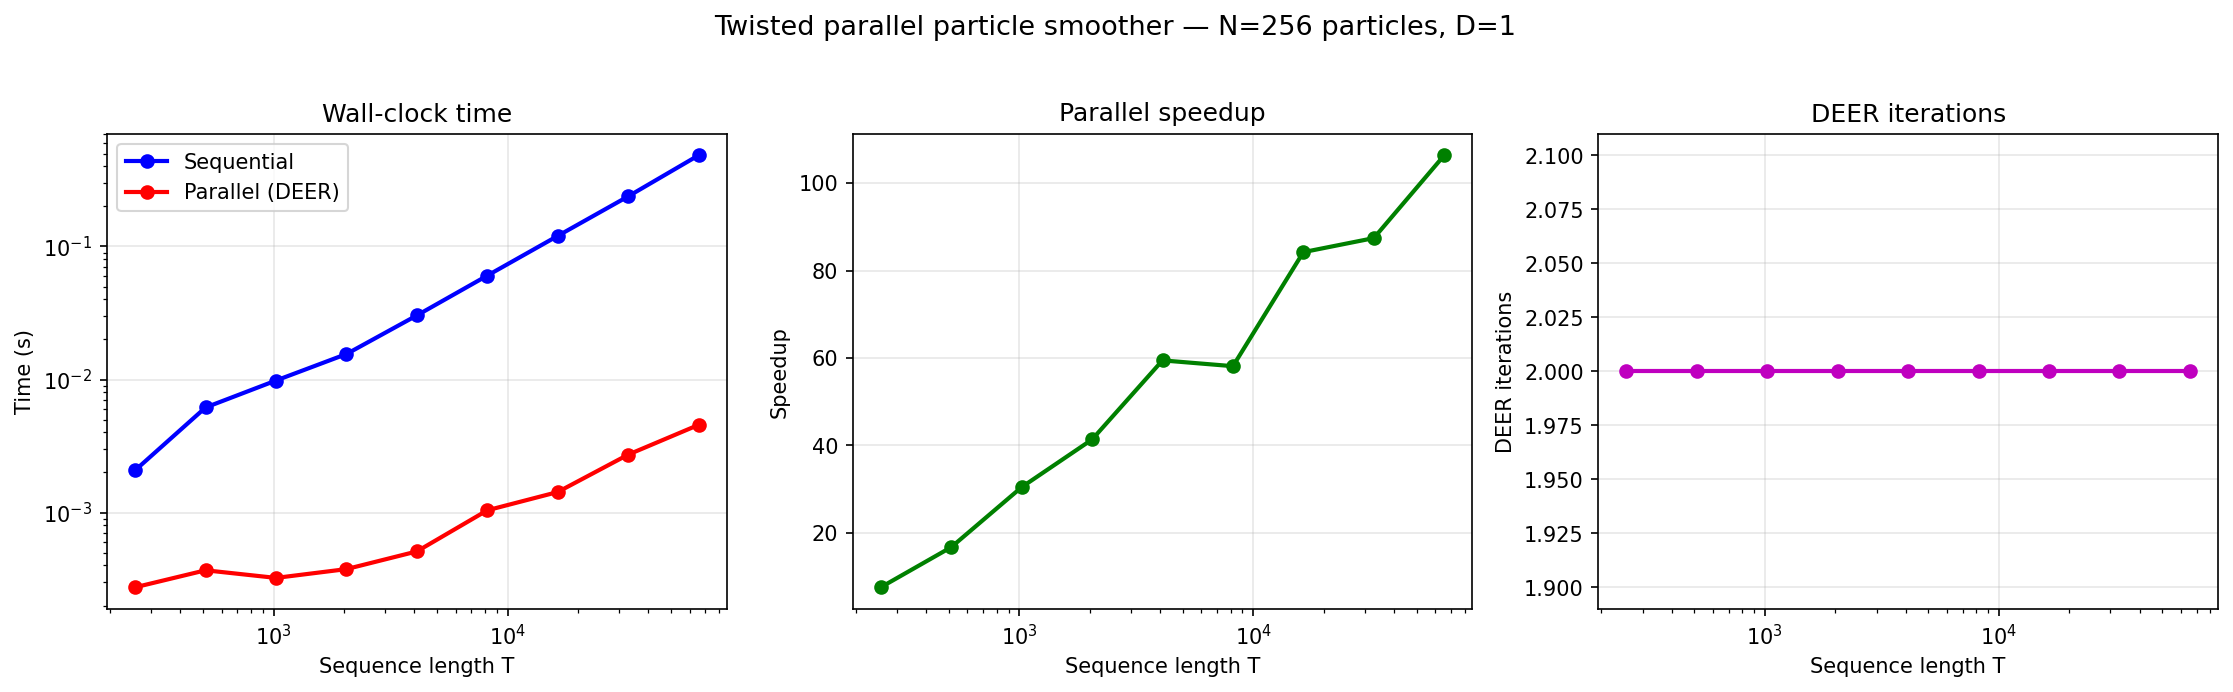
\includegraphics[width=0.95\linewidth]{../twisted_pf_scaling.png}
    \caption{Scaling in trajectory length $T$ on a $D=1, N=256$ LGSSM. Parallel wall-clock (left) is essentially flat in $T$ while sequential is linear, producing speedups (middle) that grow with $T$. DEER converges in $2$ iterations independent of $T$ (right), as expected for a linearly-Gaussian recurrence.}
    \label{fig:scaling-T}
\end{figure}

\begin{table}[t]
\caption{Scaling of the twisted parallel particle smoother. \textbf{Left:} $T$ sweep on a $D=1$ LGSSM with $N=256$. \textbf{Middle:} $D$ sweep at $T=4096, N=256$, comparing independent and coupled latent dynamics. \textbf{Right:} $N$ sweep at $T=4096, D=1$. Speedup is sequential / parallel wall-clock; parallel and sequential RMSE agree to four significant figures throughout.}
\label{tab:scaling-T}
\centering
\small
\begin{tabular}{rrrr}
\toprule
$T$ & $t_{\text{seq}}$ (s) & $t_{\text{par}}$ (s) & speedup \\
\midrule
$256$    & $0.0018$ & $0.0002$ & $9.5\times$  \\
$1024$   & $0.0071$ & $0.0003$ & $24.2\times$ \\
$4096$   & $0.0283$ & $0.0003$ & $86.8\times$ \\
$16384$  & $0.1099$ & $0.0005$ & $\mathbf{201.6\times}$ \\
$65536$  & $0.4482$ & $0.0034$ & $131.3\times$ \\
\bottomrule
\end{tabular}
\quad
\begin{tabular}{lrrrr}
\toprule
$D$ & type & iters & speedup \\
\midrule
$1$  & indep   & $2$ & $114.7\times$ \\
$8$  & indep   & $2$ & $8.6\times$  \\
$32$ & indep   & $2$ & $2.5\times$  \\
$1$  & coupled & $2$ & $115.5\times$ \\
$8$  & coupled & $7$ & $1.9\times$  \\
$32$ & coupled & $7$ & $0.6\times$  \\
\bottomrule
\end{tabular}
\quad
\begin{tabular}{rrr}
\toprule
$N$ & speedup & RMSE \\
\midrule
$16$   & $145.5\times$ & $0.124$ \\
$256$  & $92.3\times$ & $0.032$ \\
$1024$ & $55.7\times$ & $0.016$ \\
$2048$ & $20.5\times$ & $0.012$ \\
\bottomrule
\end{tabular}
\end{table}

\paragraph{Scaling in $D$, with a fix for coupled dynamics.} Figure~\ref{fig:scaling-DN} (top) characterizes the limits of the diagonal-Hutchinson Jacobian. When latent dimensions evolve independently, DEER stays at $2$ iterations and speedup degrades only with per-step compute ($114.7\times$ at $D=1$, $2.5\times$ at $D=32$). When latent dimensions are coupled, the diagonal estimator misses off-diagonal Jacobian entries, the iteration count climbs to $6$--$7$, and parallel runtime crosses sequential at $D \approx 16$. We \emph{recover} this regime with a full $(D,D)$-block Jacobian scan (Table~\ref{tab:fulljac}): on the same coupled benchmark at $T=4096, N=128$, the full-Jacobian variant converges in $\mathbf{2}$ iterations across $D \in \{4, 8, 16, 32\}$, restoring speedups of $\mathbf{12\times}$--$\mathbf{37\times}$. The associative scan operator becomes a $(D,D)$ matmul of cost $O(D^2)$, which dominates beyond $D \approx 64$.

\begin{table}[t]
\caption{Full-Jacobian DEER recovers coupled-dynamics performance ($T=4096$, $N=128$). The diagonal-Hutchinson approximation misses off-diagonal Jacobian entries and stalls at $7$ iterations; the full $(D,D)$-block scan converges in $2$ iterations at all tested dimensions and restores order-of-magnitude speedups.}
\label{tab:fulljac}
\centering
\small
\begin{tabular}{rrrrrr}
\toprule
$D$ & diag iters & diag speedup & full-Jac iters & full-Jac speedup & RMSE gain \\
\midrule
$4$  & $7$ & $13.2\times$ & $\mathbf{2}$ & $\mathbf{37.1\times}$ & $36\times$ \\
$8$  & $7$ & $4.5\times$  & $\mathbf{2}$ & $\mathbf{34.3\times}$ & $28\times$ \\
$16$ & $7$ & $1.9\times$  & $\mathbf{2}$ & $\mathbf{16.5\times}$ & $36\times$ \\
$32$ & $7$ & $1.4\times$  & $\mathbf{2}$ & $\mathbf{12.0\times}$ & $47\times$ \\
\bottomrule
\end{tabular}
\end{table}

\paragraph{Scaling in $N$.} Particle-count scaling (Figure~\ref{fig:scaling-DN} bottom; Table~\ref{tab:scaling-T} right) is benign: parallel time grows sublinearly in $N$ because particles share the device, so speedup decays from $145.5\times$ at $N{=}16$ to $20.5\times$ at $N{=}2048$ while RMSE drops from $0.124$ to $0.012$ as $N^{-1/2}$. This gives the user a clean knob to trade wall-clock for estimator variance.

\begin{figure}[t]
    \centering
    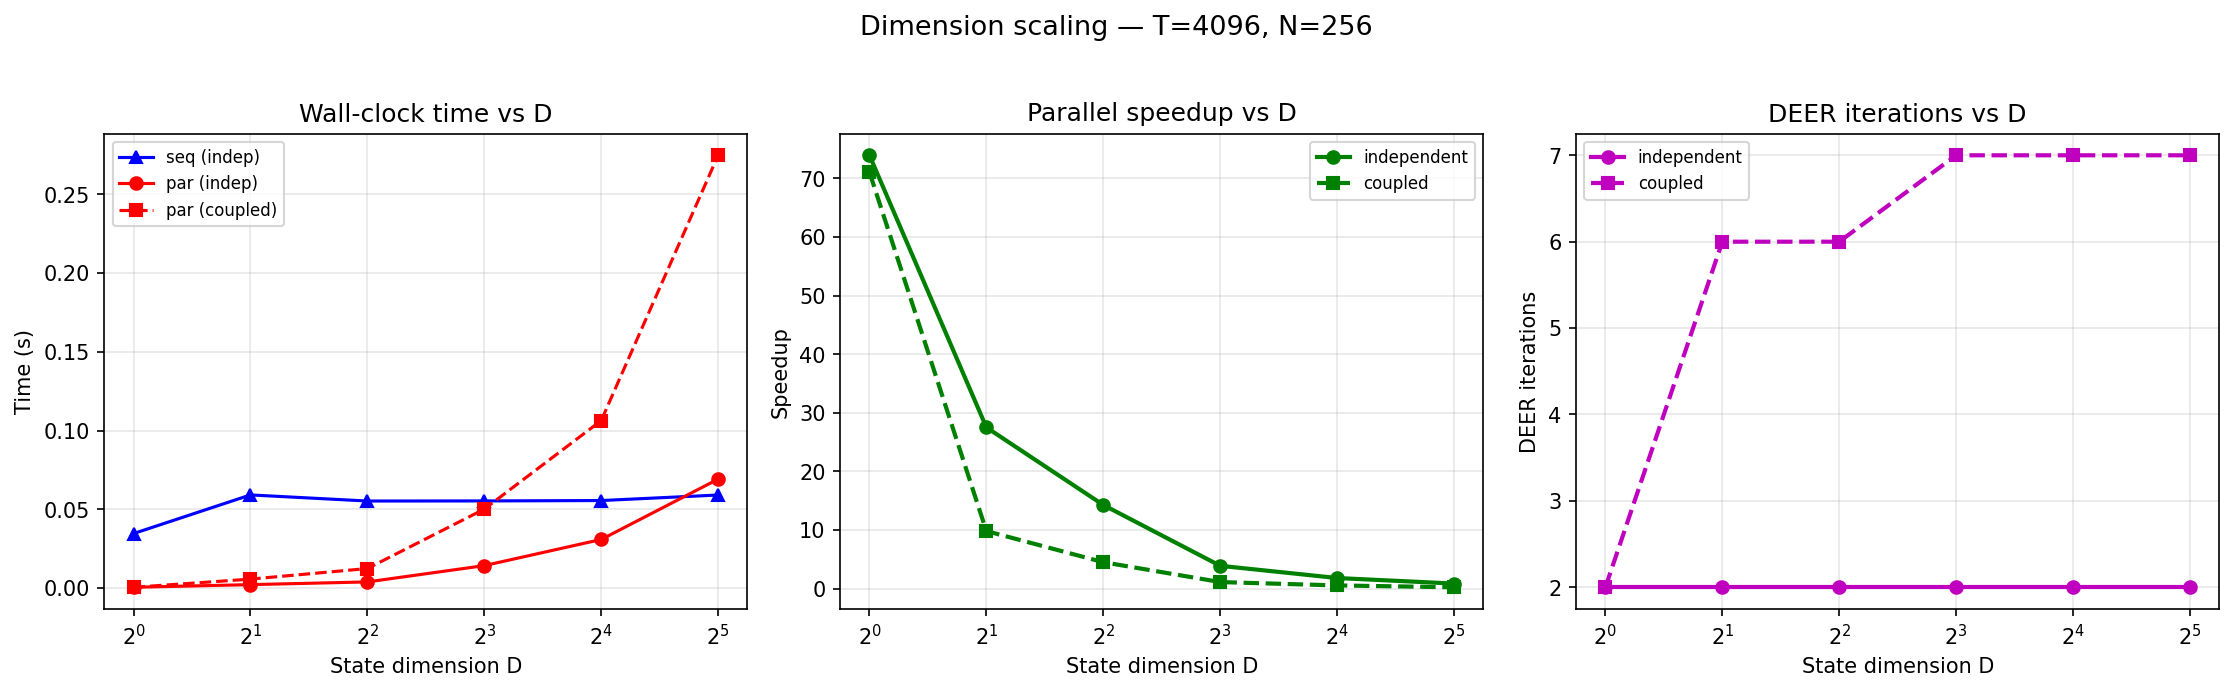
\includegraphics[width=0.95\linewidth]{../twisted_pf_scaling_D.png}\\[0.5em]
    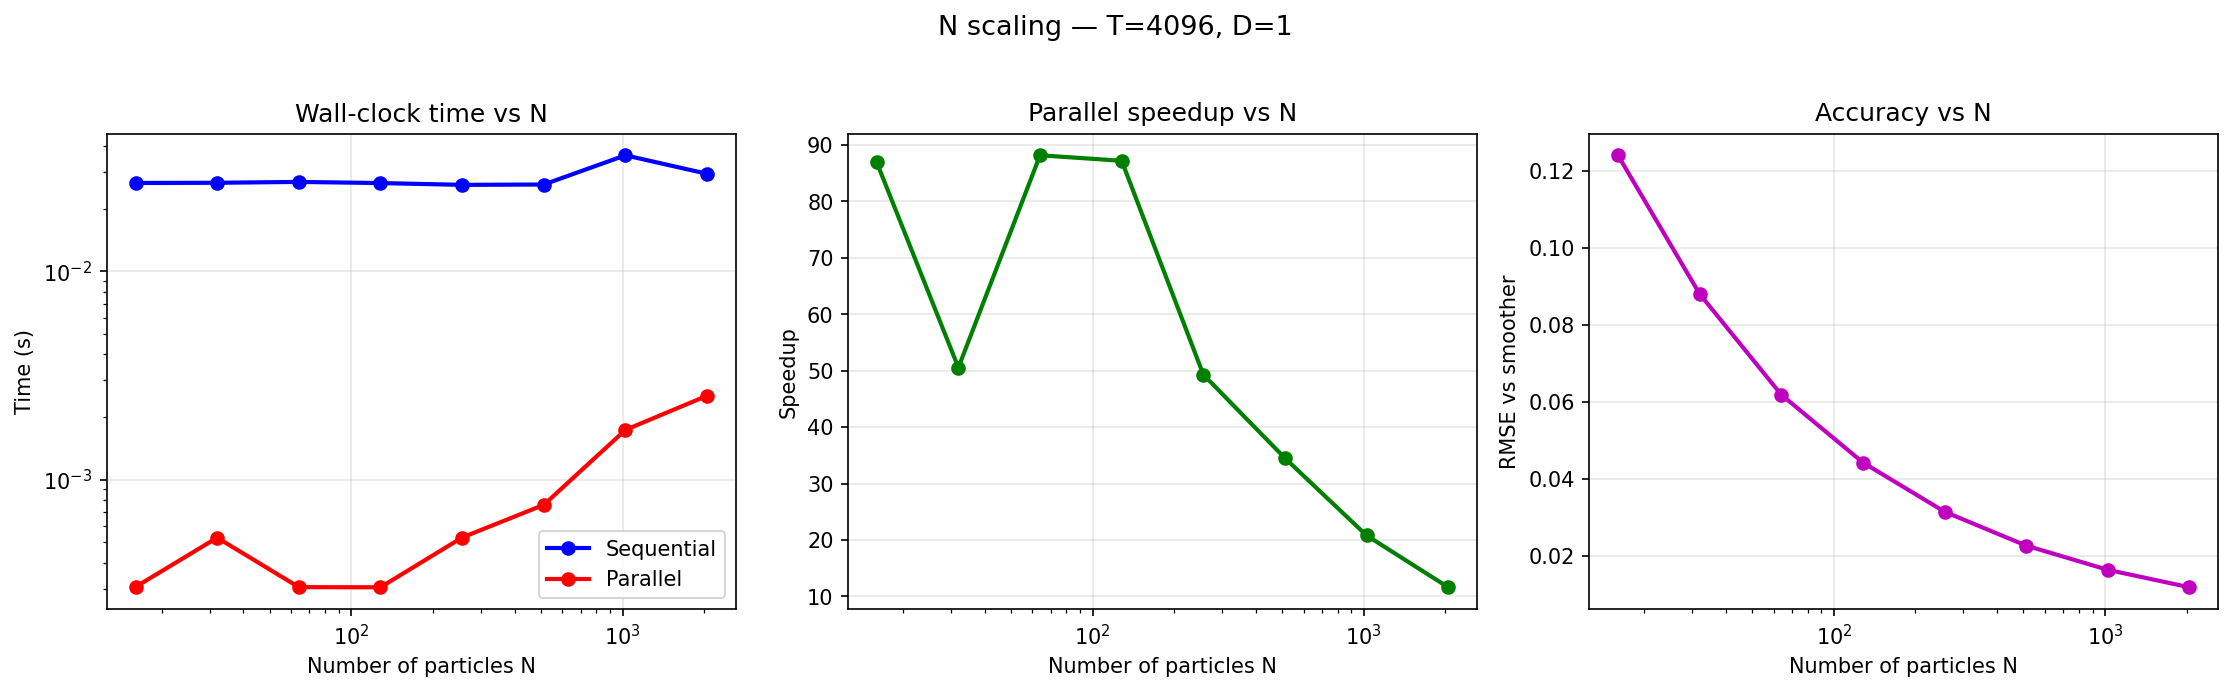
\includegraphics[width=0.95\linewidth]{../twisted_pf_scaling_N.png}
    \caption{Scaling in latent dimension $D$ (top) and particle count $N$ (bottom). With diagonal-Hutchinson Jacobians, independent dimensions stay at the $2$-iteration floor (top right) and degrade gracefully; coupled dimensions hit $6$--$7$ iterations and parallel runtime crosses sequential near $D=16$. Particle-count scaling is benign: speedup decays smoothly with $N$ while RMSE shrinks as $N^{-1/2}$ (bottom right).}
    \label{fig:scaling-DN}
\end{figure}

\subsubsection{Parallelism is essentially free; twist quality is the bottleneck}
\label{sec:exp-twist-ablation}

\paragraph{C2.} Figure~\ref{fig:twist-ablation} and Table~\ref{tab:twist-ablation} sweep the twist on a $T=4096$ LGSSM at $N=256$. All four twists hit DEER's $2$-iteration floor---the linearization is exact for Gaussian dynamics regardless of twist---and the parallel speedup is essentially constant at $58\times$--$66\times$. What changes by an order of magnitude is the smoother's \emph{statistical} quality: the prior twist gives effective sample size (ESS) of $1.0/256$ and RMSE $1.37$, while the BIF-smoother twist achieves $\text{ESS}=3.2/256$ and RMSE $\mathbf{0.041}$---a $33\times$ RMSE improvement at no parallel cost. \textit{Parallelism comes from the recurrence structure; estimator variance is governed entirely by twist quality.} Subsequent experiments therefore use learned look-ahead twists.

\begin{figure}[t]
    \centering
    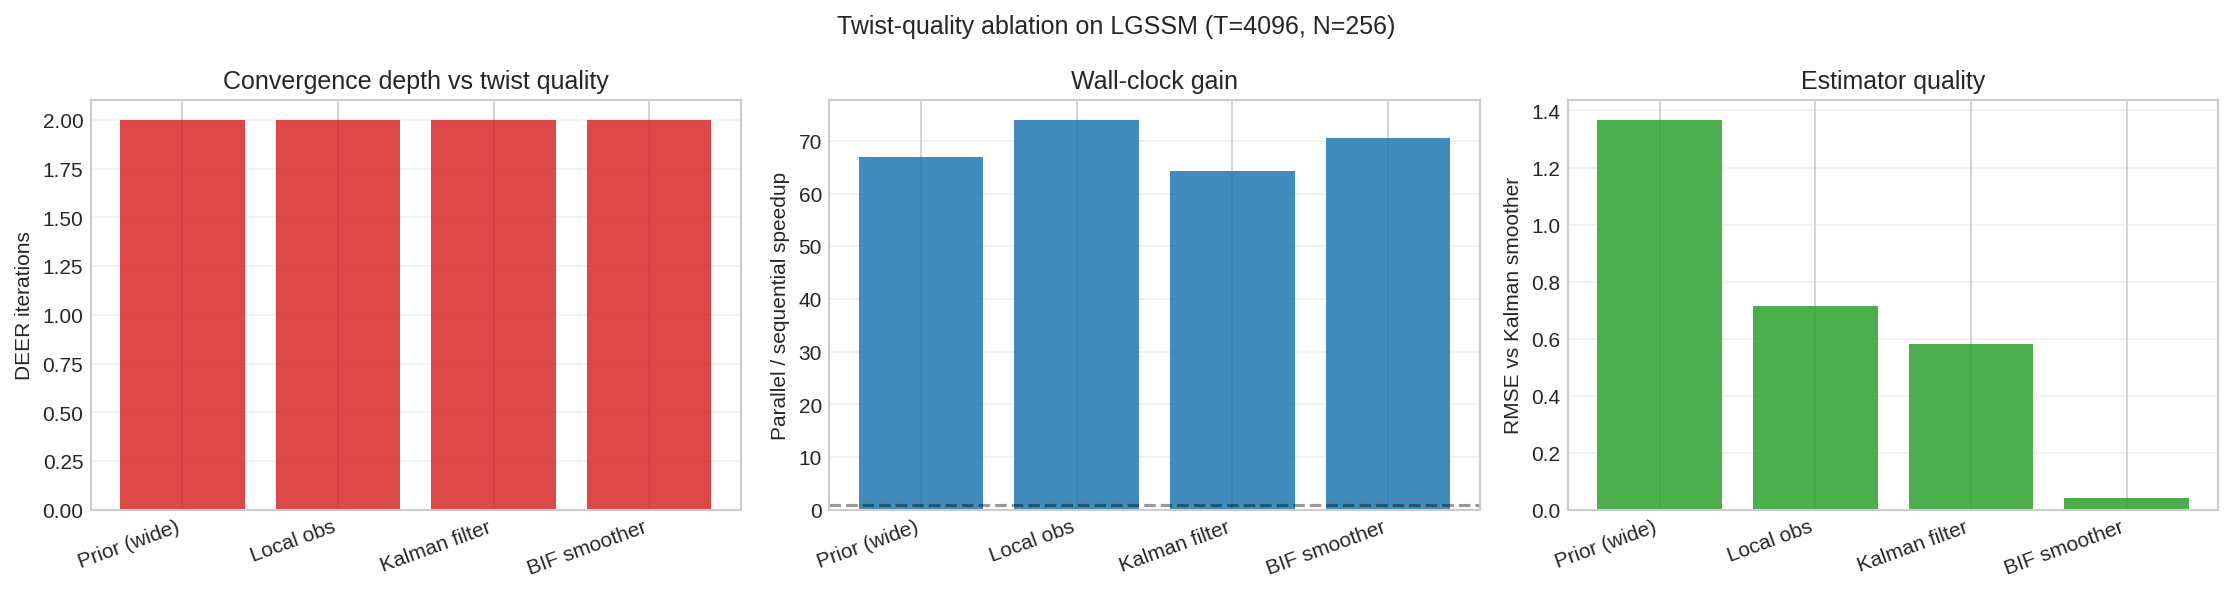
\includegraphics[width=0.95\linewidth]{../twist_ablation.png}
    \caption{Twist-quality ablation on LGSSM ($T=4096, N=256$). All four twists hit DEER's $2$-iteration floor (left) with comparable wall-clock speedup (middle), but their statistical quality (right) varies by more than an order of magnitude: a wide prior twist yields RMSE $1.37$ vs.\ $0.04$ for a backward-information-filter twist. Parallelism is essentially free; twist quality is the bottleneck.}
    \label{fig:twist-ablation}
\end{figure}

\begin{table}[t]
\caption{Twist quality ablation on LGSSM ($T=1000, D=1, N=256$). All twists hit DEER's $2$-iteration floor, so wall-clock speedup is constant; ESS and RMSE separate strong twists from weak ones by $> 30\times$.}
\label{tab:twist-ablation}
\centering
\small
\begin{tabular}{lrrrrr}
\toprule
Twist & DEER iters & $t_{\text{seq}}$ (ms) & $t_{\text{par}}$ (ms) & speedup & RMSE \\
\midrule
Prior (wide)        & $2$ & $29.5$ & $0.51$ & $57.9\times$ & $1.367$ \\
Local obs           & $2$ & $30.8$ & $0.48$ & $64.3\times$ & $0.716$ \\
Kalman filter       & $2$ & $30.8$ & $0.47$ & $66.1\times$ & $0.582$ \\
\textbf{BIF smoother} & $2$ & $30.6$ & $0.48$ & $64.0\times$ & $\mathbf{0.041}$ \\
\bottomrule
\end{tabular}
\end{table}

\subsubsection{Nonlinear and chaotic dynamics}
\label{sec:exp-nonlinear}

\paragraph{C3a. Stochastic volatility.} The stochastic volatility model has a nonlinear observation $y_t \mid x_t \sim \mathcal{N}(0, \beta^2 e^{x_t})$ that does not admit a closed-form look-ahead. We learn the twist by ELBO maximization over a small mean-and-log-scale network: $500$ steps of Adam in $10.5$s. The trained twist drives the parallel smoother to a sequential-bit-equal RMSE of $0.566$ in $0.3$ms vs.\ $5.7$ms sequentially---a $\mathbf{18.9\times}$ speedup at $2$ DEER iterations. The same architecture, amortized over $\theta$ rather than fit to a single $\theta$, drives STAMPEDE in \S\ref{sec:exp-mcmc}.

\paragraph{C3b. Lorenz-63: full-covariance twists capture posterior coupling.} On the chaotic Lorenz-63 system ($T=2000, D=3, N=512$), the smoothing posterior has strong $(x,y,z)$ coupling that a diagonal twist cannot represent. Table~\ref{tab:lorenz63} and Figure~\ref{fig:lorenz63} compare an extended-Kalman analytic twist to a learned full-covariance neural twist parameterized as $\psi_t(x) = \mathcal{N}(\mu_t, L_t L_t^\top)$ with Cholesky $L_t$. The learned full-cov twist matches the EKF smoother RMSE ($0.684$) and \emph{beats} bootstrap PS/FFBSi ($0.696$); the EKF-twist variant runs at $6\times$ parallel speedup with $8$ DEER iterations. The learned twist requires $\rho=0.95$ DEER damping (\S\ref{sec:twist-damping}): the effective Jacobian $\Sigma_{\text{post}} J_q^{-1} J_f$ has complex eigenvalues of magnitude $\approx 0.91$, and without damping the iteration fails to converge. With damping we obtain $2.8\times$ parallel speedup at $30$ iterations---lower than for Gaussian models, but the only method that matches EKF-smoother accuracy in tens of milliseconds.

\begin{figure}[t]
    \centering
    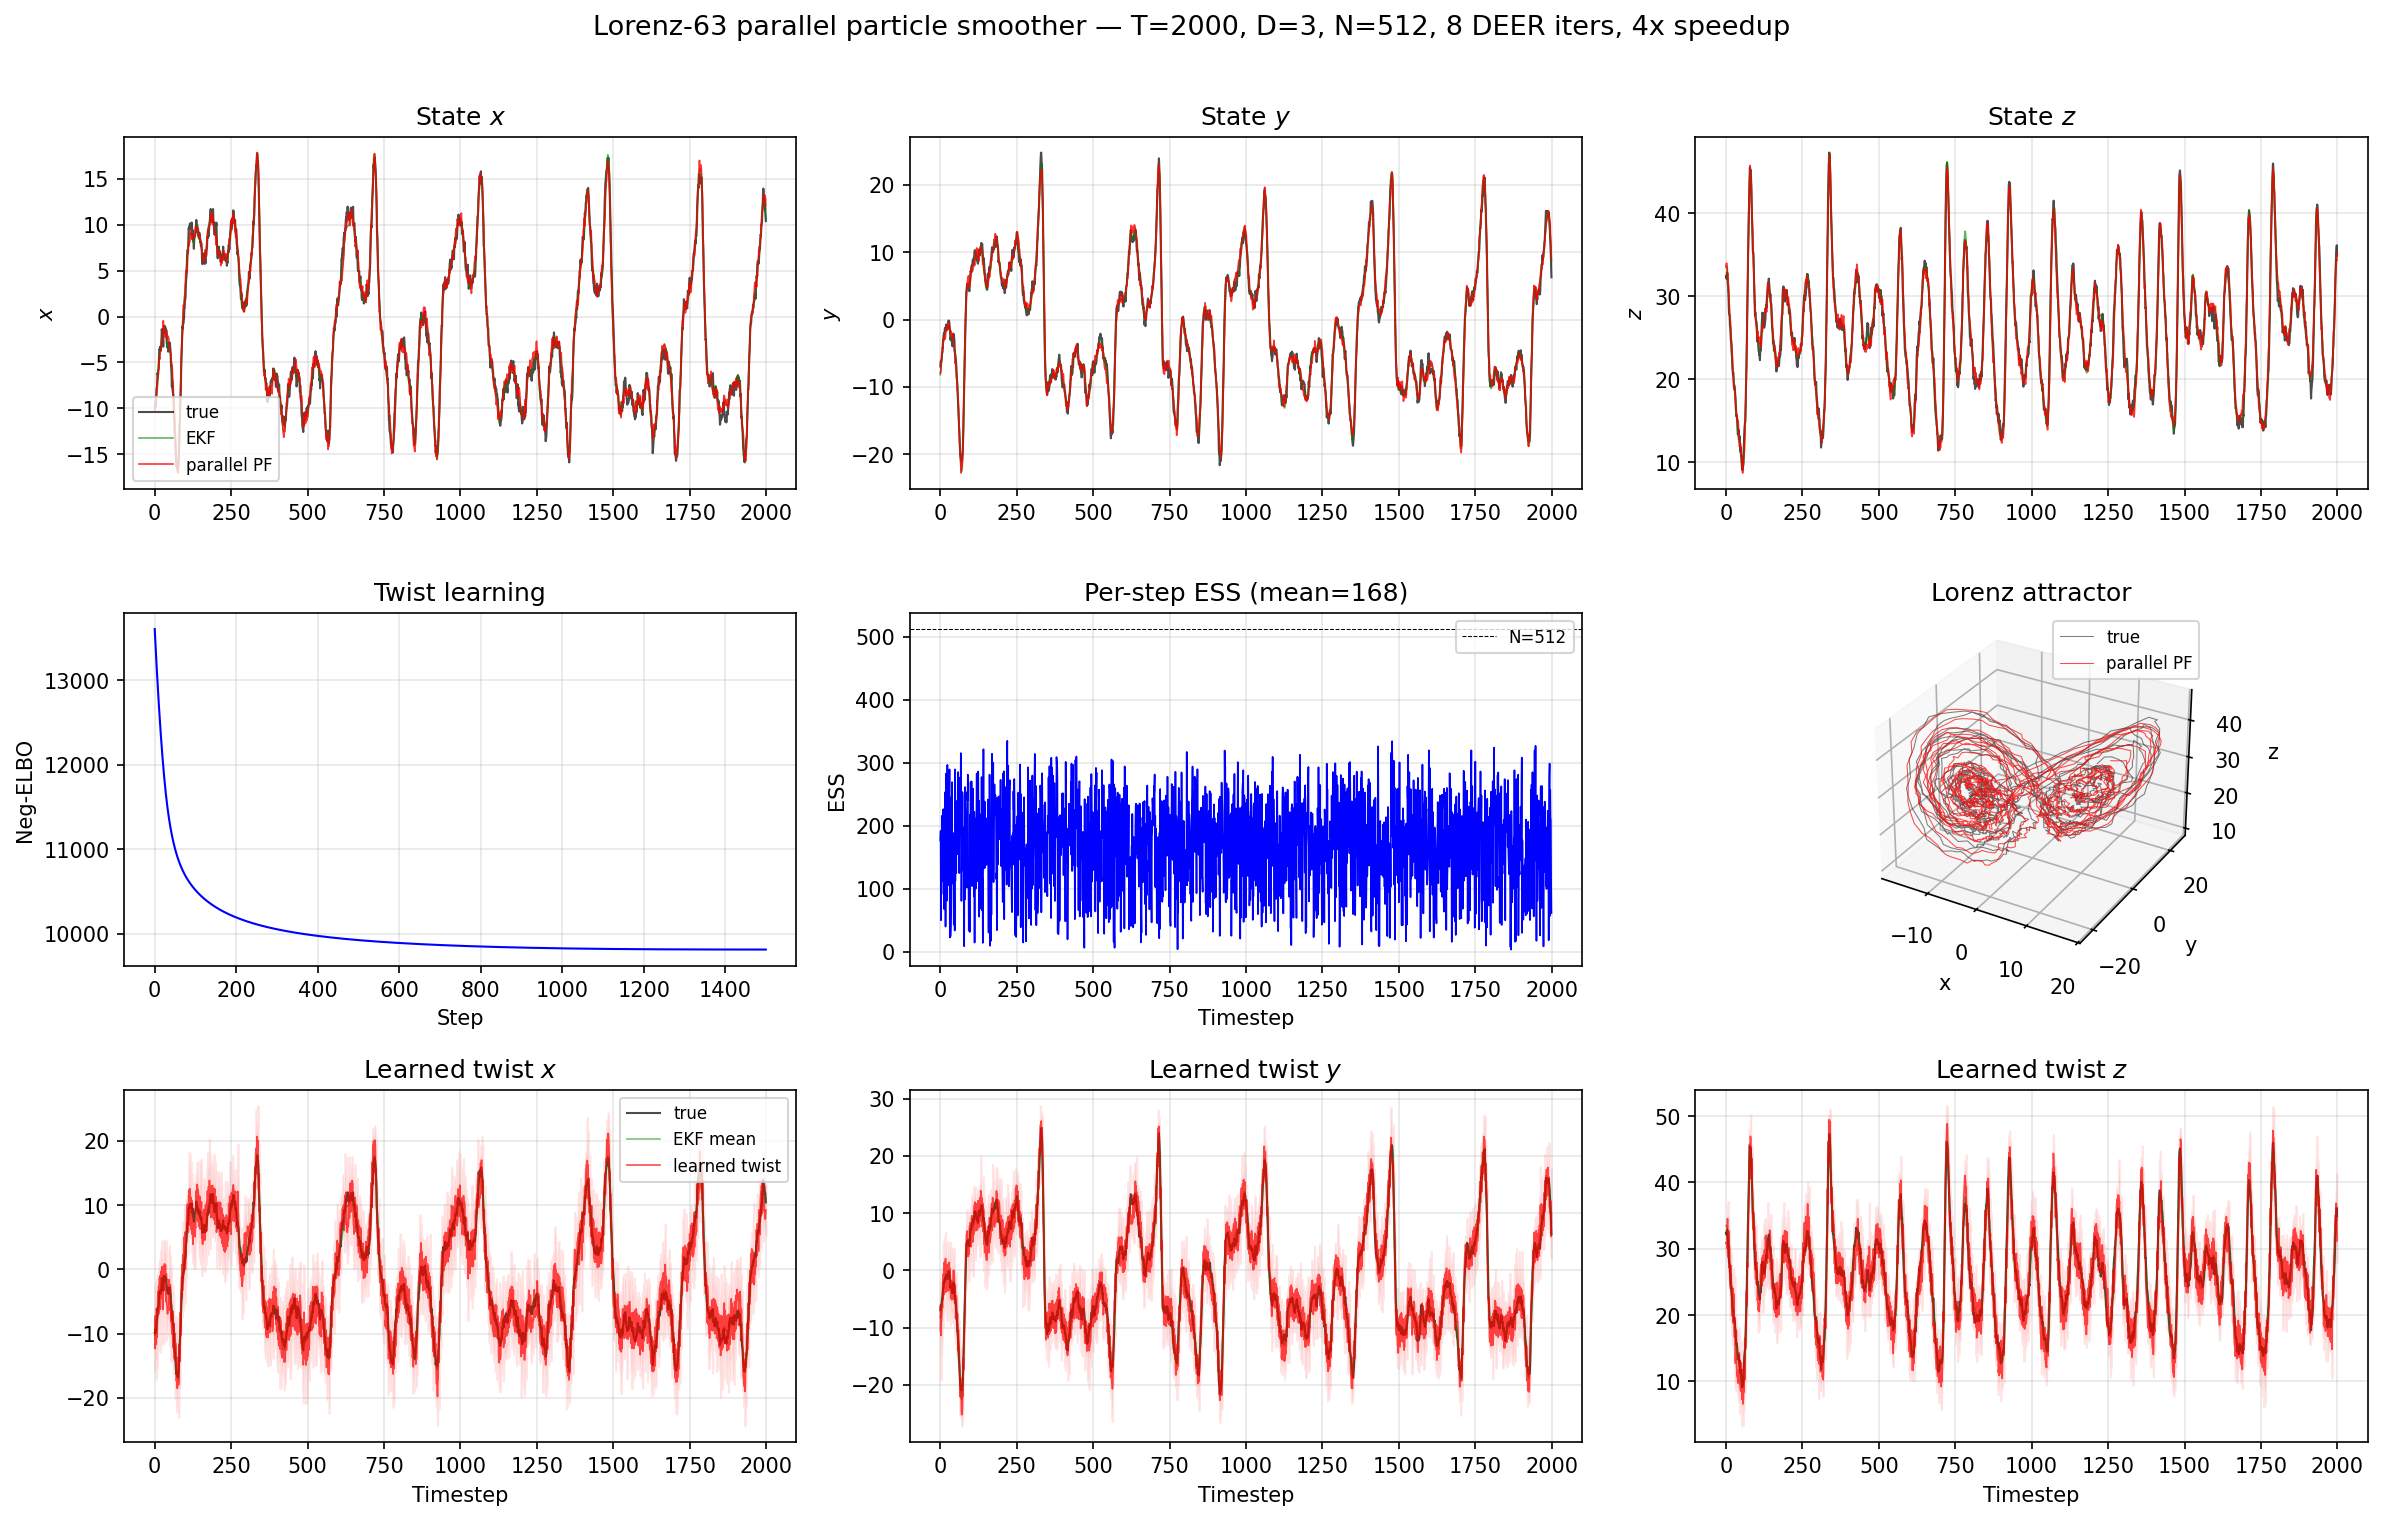
\includegraphics[width=0.95\linewidth]{../twisted_pf_lorenz63.png}
    \caption{Lorenz-63 parallel particle smoother ($T=2000, D=3, N=512$). Top row: state-component trajectories (true vs.\ smoothed). Middle row: twist-network ELBO training curve, per-step ESS, and 3D Lorenz attractor. Bottom row: the learned full-covariance twist's mean tracks the EKF smoother mean across $(x,y,z)$, capturing the cross-component coupling that a diagonal twist would miss.}
    \label{fig:lorenz63}
\end{figure}

\begin{table}[t]
\caption{Lorenz-63 smoothing ($T=2000, D=3, N=512$). The learned full-covariance neural twist matches the EKF smoother (the analytic reference) and beats FFBSi by a wide margin in RMSE, while the parallel implementation cuts wall-clock by $2.8\times$ over the sequential twisted version.}
\label{tab:lorenz63}
\centering
\small
\begin{tabular}{lrrrr}
\toprule
Method & Time (s) & RMSE & DEER iters & Speedup vs.\ seq \\
\midrule
EKF smoother (reference)        & --        & $0.684$ & --   & --     \\
Bootstrap PF (filter)           & $0.188$   & $0.885$ & --   & --     \\
Bootstrap PS / FFBSi            & $0.022$   & $0.696$ & --   & --     \\
EKF twist (sequential)          & $0.153$   & $0.868$ & --   & $1.0\times$ \\
EKF twist (parallel)            & $0.026$   & $0.868$ & $8$  & $\mathbf{6.0\times}$ \\
Learned full-cov twist (seq)    & $0.149$   & $0.684$ & --   & $1.0\times$ \\
\textbf{Learned full-cov twist (parallel)} & $\mathbf{0.053}$ & $\mathbf{0.684}$ & $30$ & $\mathbf{2.8\times}$ \\
\bottomrule
\end{tabular}
\end{table}

\paragraph{C3c. Lorenz-96: bootstrap baselines collapse, twisted smoother holds.} To stress the method beyond $D=3$ we run Lorenz-96 ($T=2000$, $N=64$, $F=8$ forcing) at $D \in \{10, 20, 40\}$ using full-Jacobian DEER. Figure~\ref{fig:lorenz96} and Table~\ref{tab:lorenz96} make a striking comparison: the twisted smoother's RMSE stays \emph{flat} at $0.29$--$0.30$ as $D$ grows, while bootstrap PF and FFBSi degrade from $\approx 0.39$ at $D=10$ to $2.70$ at $D=40$, an order of magnitude worse and a regime where the bootstrap chain is providing essentially no information. The parallel implementation matches sequential RMSE bit-for-bit and runs $1.5\times$ faster at $D=10$; at $D=20, 40$ the $O(D^2)$ scan cost outpaces the depth advantage at this $T$, so parallel and sequential have comparable wall-clock---but both \emph{dominate} bootstrap baselines on the RMSE Pareto frontier. For high-dimensional chaotic systems the twisted smoother is a clean \emph{statistical} win at no wall-clock cost over its sequential reference.

\begin{figure}[t]
    \centering
    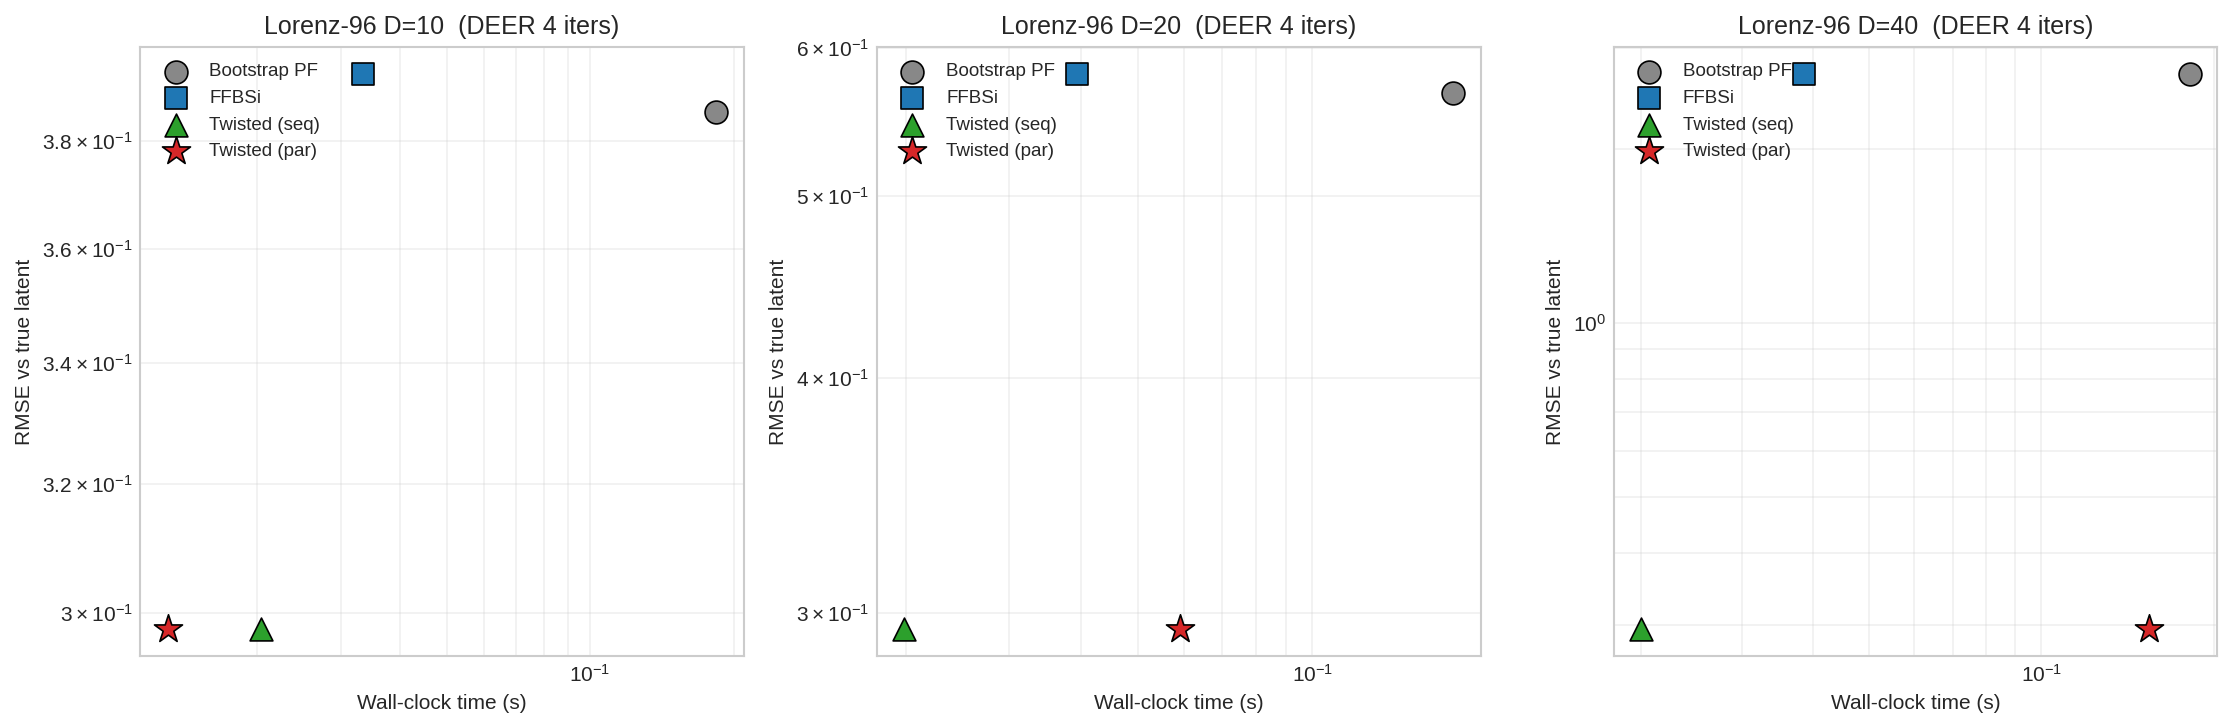
\includegraphics[width=0.95\linewidth]{../twisted_pf_lorenz96.png}
    \caption{Lorenz-96 RMSE versus wall-clock at $D \in \{10, 20, 40\}$ ($T=2000, N=64$). The twisted smoother (sequential triangle, parallel star) maintains an essentially constant RMSE of $\approx 0.30$ as $D$ grows, while bootstrap PF and FFBSi degrade by an order of magnitude. The parallel point sits to the right of the sequential point at $D=20, 40$: a $0.3\times$/$0.1\times$ wall-clock slowdown that nevertheless dominates both baselines on the Pareto frontier.}
    \label{fig:lorenz96}
\end{figure}

\begin{table}[t]
\caption{Lorenz-96 smoothing ($T=2000, N=64$, full-Jacobian DEER, $4$ iterations). The twisted smoother's RMSE is essentially independent of $D$, while bootstrap PF and FFBSi degrade sharply; parallel speedup, however, becomes unfavorable beyond $D=10$ as the $O(D^2)$ scan cost dominates.}
\label{tab:lorenz96}
\centering
\small
\begin{tabular}{rrrrrr}
\toprule
$D$ & BPF RMSE & FFBSi RMSE & Twisted RMSE & $t_{\text{seq}} / t_{\text{par}}$ & Speedup vs.\ seq \\
\midrule
$10$ & $0.386$ & $0.393$ & $\mathbf{0.298}$ & $0.019$s / $0.013$s & $1.5\times$ \\
$20$ & $0.567$ & $0.581$ & $\mathbf{0.294}$ & $0.019$s / $0.060$s & $0.3\times$ \\
$40$ & $2.696$ & $2.697$ & $\mathbf{0.295}$ & $0.020$s / $0.154$s & $0.1\times$ \\
\bottomrule
\end{tabular}
\end{table}

\subsection{Drop-in E-step: particle EM for a Poisson LDS}
\label{sec:exp-em}

\paragraph{C4 (non-MCMC).} The twisted-DEER smoother is not specific to MCMC---any algorithm that needs smoothed sufficient statistics can use it as a faster E-step. We run \emph{particle EM} on a $D=5$ Poisson linear dynamical system, $x_t = A x_{t-1} + \sigma_q \epsilon_t$, $y_{t,d} \sim \text{Poisson}(\exp(x_{t,d}))$, with $T=2000$, $N=256$, and $50$ EM iterations. The E-step computes smoothed expected outer products and the M-step is closed-form least squares for $(A, \sigma_q)$. Per-iteration E-step costs at convergence are: bootstrap PF $0.20$s, FFBSi $0.034$s, sequential twisted $0.185$s, parallel twisted $\mathbf{0.007}$s---a $\mathbf{26\times}$ E-step speedup over sequential twisted and $5.1\times$ over FFBSi at comparable smoothing RMSE ($\approx 0.4$). End-to-end, parallel particle EM completes in $\mathbf{23.3}$s versus $168.6$s for the sequential twisted EM, a $\mathbf{7.2\times}$ wall-clock improvement. (Implementation note: a naive parallel E-step inside a Python EM loop \emph{regresses} to $0.4\times$ because each call retraces the JAX program; JIT-wrapping the full E-step recovers the headline number.)

\subsection{STAMPEDE for parameter inference}
\label{sec:exp-mcmc}

\paragraph{C4. Setup and baselines.} We compare STAMPEDE against (i) standard pseudo-marginal MCMC with a bootstrap PF likelihood and random-walk Metropolis proposals (``Standard PMCMC''), and (ii) sequential twisted PMCMC with frozen-randomness MALA proposals (``Twisted seq''). The Twisted-seq baseline isolates the contribution of the outer DEER scan: any speedup of STAMPEDE over Twisted seq is attributable to chain-index parallelism alone, while the gap to Standard PMCMC reflects the combined effect of twisting, gradient information, and parallelism. We evaluate on a linear-Gaussian benchmark and a stochastic volatility model.

\paragraph{Amortized twist for parameter inference.} A subtle but important point is that the twist must generalize over $\theta$, not just be tuned at a single $\theta$. We parameterize $\psi_t(x; \theta) = \mathcal{N}(\mu_\phi(t, \theta), \exp(\ell_\phi(t, \theta)))$ as a small neural network (two hidden layers, $128$ units, shared across $t$) and train in two phases: (1) a BIF-target warm-start fitting the network to analytic backward-information-filter targets at $512$ random $\theta$ draws ($666$ Adam steps, $\sim 60$s); (2) ELBO fine-tuning of the marginal-likelihood lower bound at the same $\theta$ samples ($1334$ Adam steps with $64$-particle SMC unrolls, $\sim 125$s). Total amortization cost is $\sim 185$s, paid \emph{once} before MCMC. At test time the network is frozen and called as a deterministic function of $(t, \theta)$ inside both the inner DEER scan and the outer MALA gradient.

\begin{table}[t]
\caption{STAMPEDE vs.\ baselines for parameter inference. All experiments use the same chain length $K$ and the same posterior-fidelity diagnostics; STAMPEDE wins on wall-clock against both baselines while matching Twisted seq on bias.}
\label{tab:stampede-mcmc}
\centering
\small
\begin{tabular}{lrrrr}
\toprule
\multicolumn{1}{l}{\textbf{LGSSM}} & \multicolumn{4}{l}{$T=500, N=256, K=2000$ ($80 \times 25$ blocks)} \\
\midrule
Method & Time (s) & vs.\ Std & vs.\ TwSeq & Notes \\
\midrule
Standard PMCMC (BPF + RW)        & $89.4$ & $1.0\times$ & --          & accept $0.38$ \\
Twisted seq PMCMC (MALA)         & $54.8$ & $1.6\times$ & $1.0\times$ & accept $0.80$ \\
\textbf{STAMPEDE}                & $\mathbf{35.1}$ & $\mathbf{2.5\times}$ & $\mathbf{1.6\times}$ & $9$ DEER iters / block \\
\midrule
\multicolumn{1}{l}{\textbf{Stochastic volatility}} & \multicolumn{4}{l}{$T=1000, N=256, K=2000$ ($80 \times 25$ blocks), amortized twist} \\
\midrule
Standard PMCMC                   & $187.6$  & $1.0\times$ & --          & accept $0.42$, $\phi$-bias $4.4\sigma$ \\
Twisted seq PMCMC                & $130.3$  & $1.4\times$ & $1.0\times$ & accept $0.72$ \\
\textbf{STAMPEDE}                & $\mathbf{73.5}$ & $\mathbf{2.6\times}$ & $\mathbf{1.8\times}$ & $7$ DEER iters / block \\
\bottomrule
\end{tabular}
\end{table}

\paragraph{Linear-Gaussian state-space model.} On the LGSSM (Table~\ref{tab:stampede-mcmc} top; Figure~\ref{fig:stampede-lgssm}), STAMPEDE runs in $35.1$s versus $89.4$s for Standard PMCMC and $54.8$s for Twisted seq---a $\mathbf{2.5\times}$ speedup over the standard baseline and a $\mathbf{1.6\times}$ speedup over the sequential twisted version. The DEER block solver converges in an average of $9$ iterations across $80$ blocks of $25$ proposals each. Posterior estimates for $(\phi, \sigma_q, \sigma_r)$ agree with the Twisted-seq baseline to within $0.1\sigma$ on every parameter, confirming that the outer DEER scan does not compromise sampling quality. The remaining $\sim 1\sigma$ bias on $\phi$ and $\sigma_q$ is shared by all three methods and reflects MC error at this chain length; Standard PMCMC's apparently tighter $\sigma_q$ is in fact a sign of \emph{under}-mixing, as its accept rate of $0.38$ versus MALA's $0.80$ confirms.

\paragraph{Stochastic volatility.} The stochastic volatility experiment (Table~\ref{tab:stampede-mcmc} bottom; Figure~\ref{fig:stampede-stochvol}) is the most informative of the two. With the amortized twist of \S\ref{sec:exp-mcmc}, STAMPEDE samples in $73.5$s versus $187.6$s for Standard PMCMC and $130.3$s for Twisted seq---a $\mathbf{2.6\times}$ wall-clock speedup over the standard baseline, with $7$ DEER iterations per block on average. More striking is the bias result: Standard PMCMC has a $\mathbf{4.4\sigma}$ posterior bias on the persistence parameter $\phi$ (estimated $0.979$ vs.\ true $0.95$), while Twisted seq and STAMPEDE both recover $\phi$ to within $0.1\sigma$ of truth. The bootstrap filter's high-variance likelihood estimate causes the random-walk chain to lock onto a poorly-explored mode, and the twisted look-ahead proposal---not the parallelism---is what fixes it. STAMPEDE inherits this fix at no statistical cost while being roughly twice as fast as the sequential twisted alternative.

\begin{figure}[t]
    \centering
    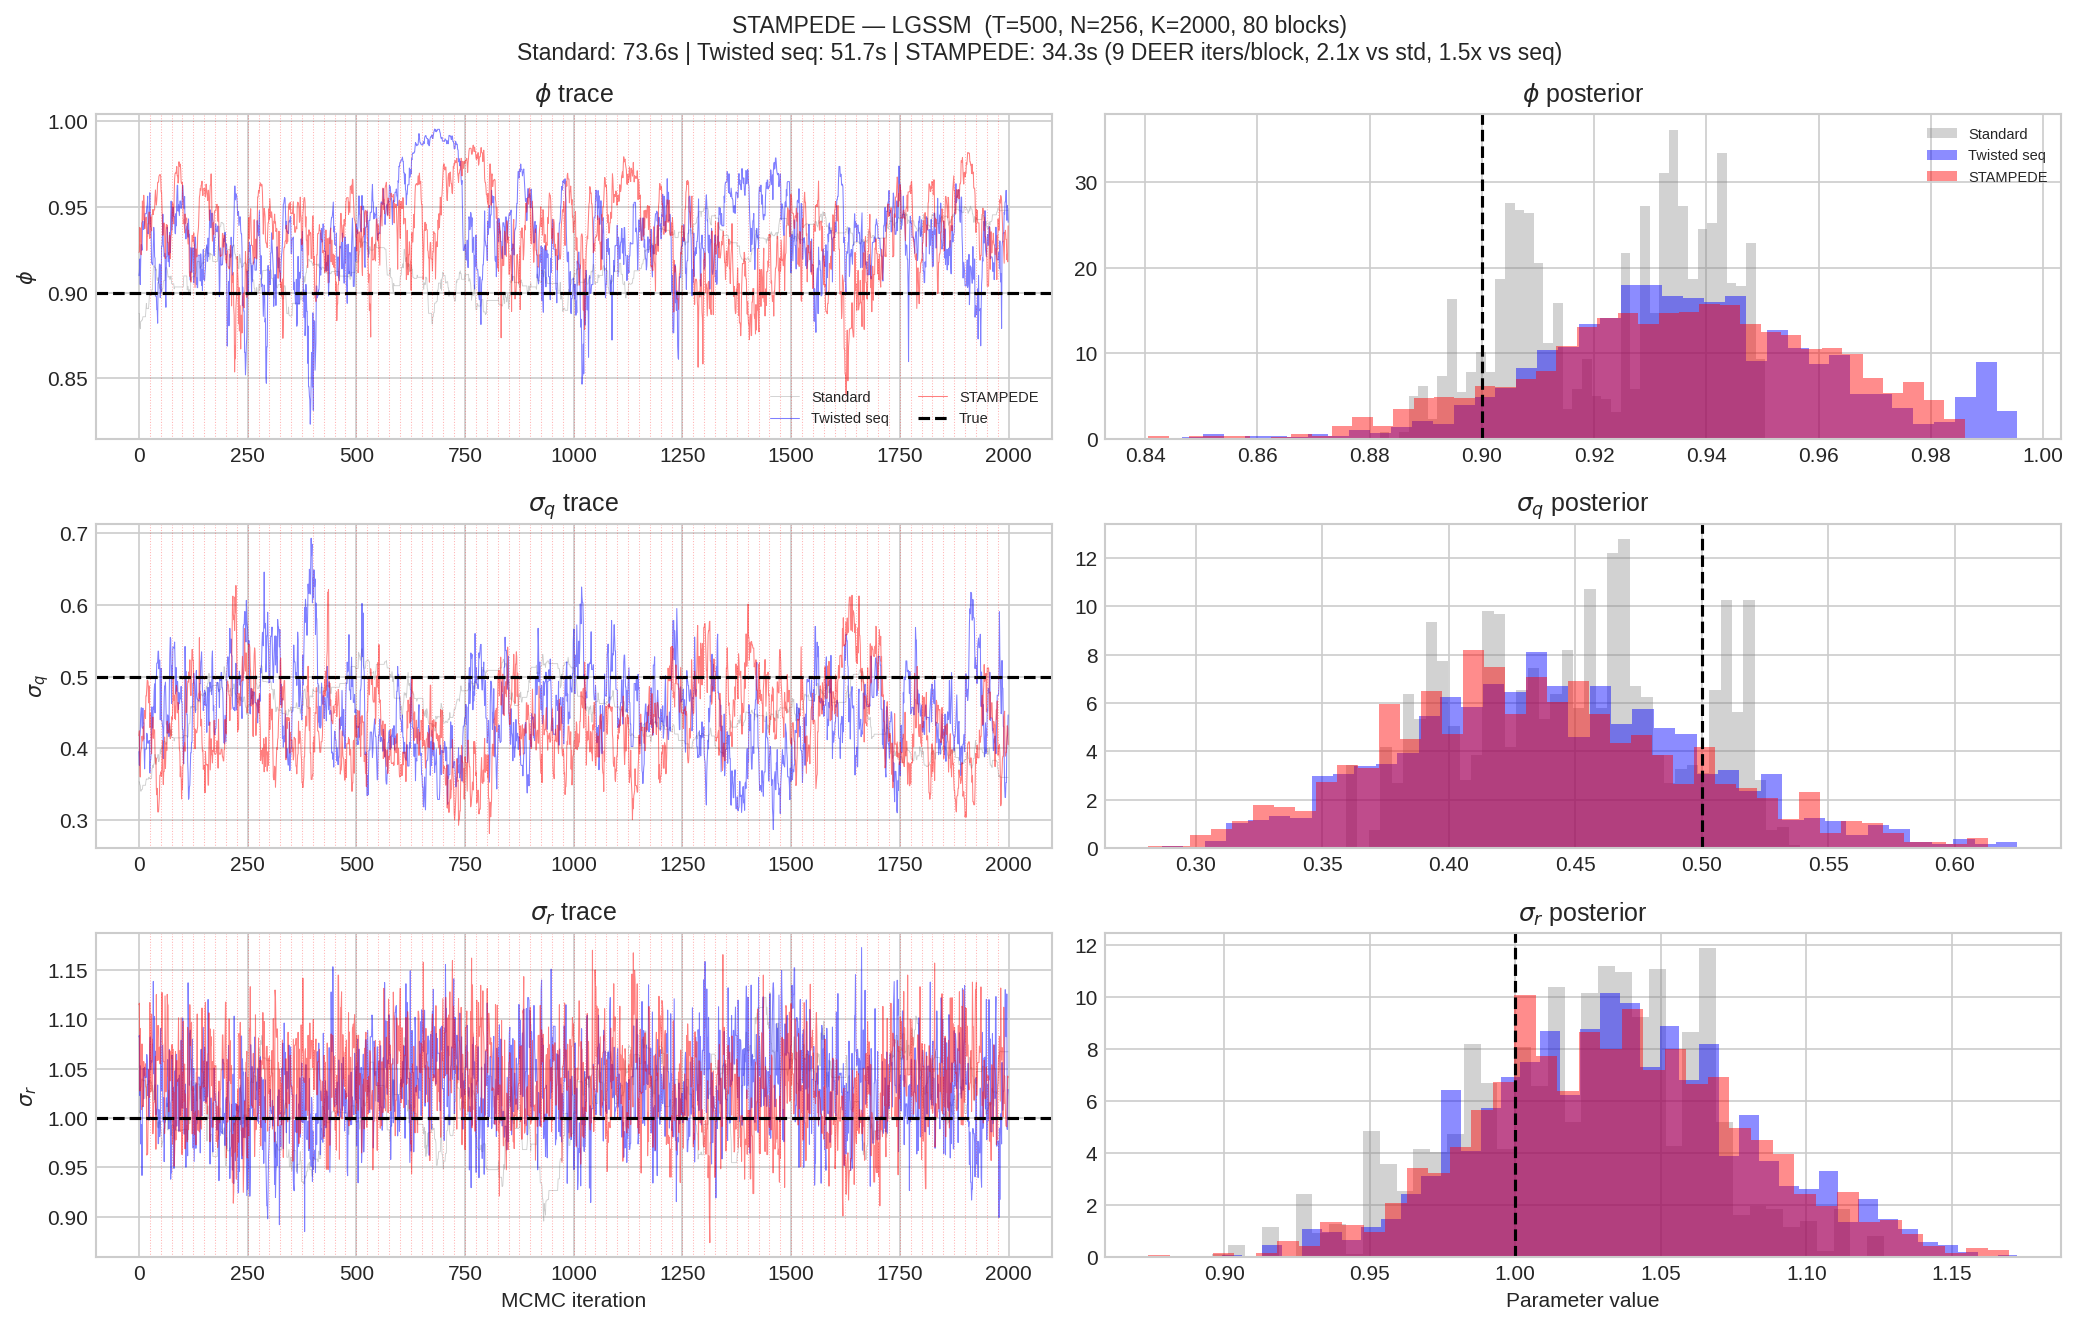
\includegraphics[width=0.92\linewidth]{../stampede_lgssm.png}
    \caption{STAMPEDE on the LGSSM ($T=500, K=2000$). Trace plots (left) show all three samplers exploring the same posterior; histograms (right) confirm that STAMPEDE and Twisted seq match each other to within MC error, while Standard PMCMC's narrower $\phi$ histogram is a symptom of under-mixing rather than higher accuracy.}
    \label{fig:stampede-lgssm}
\end{figure}

\begin{figure}[t]
    \centering
    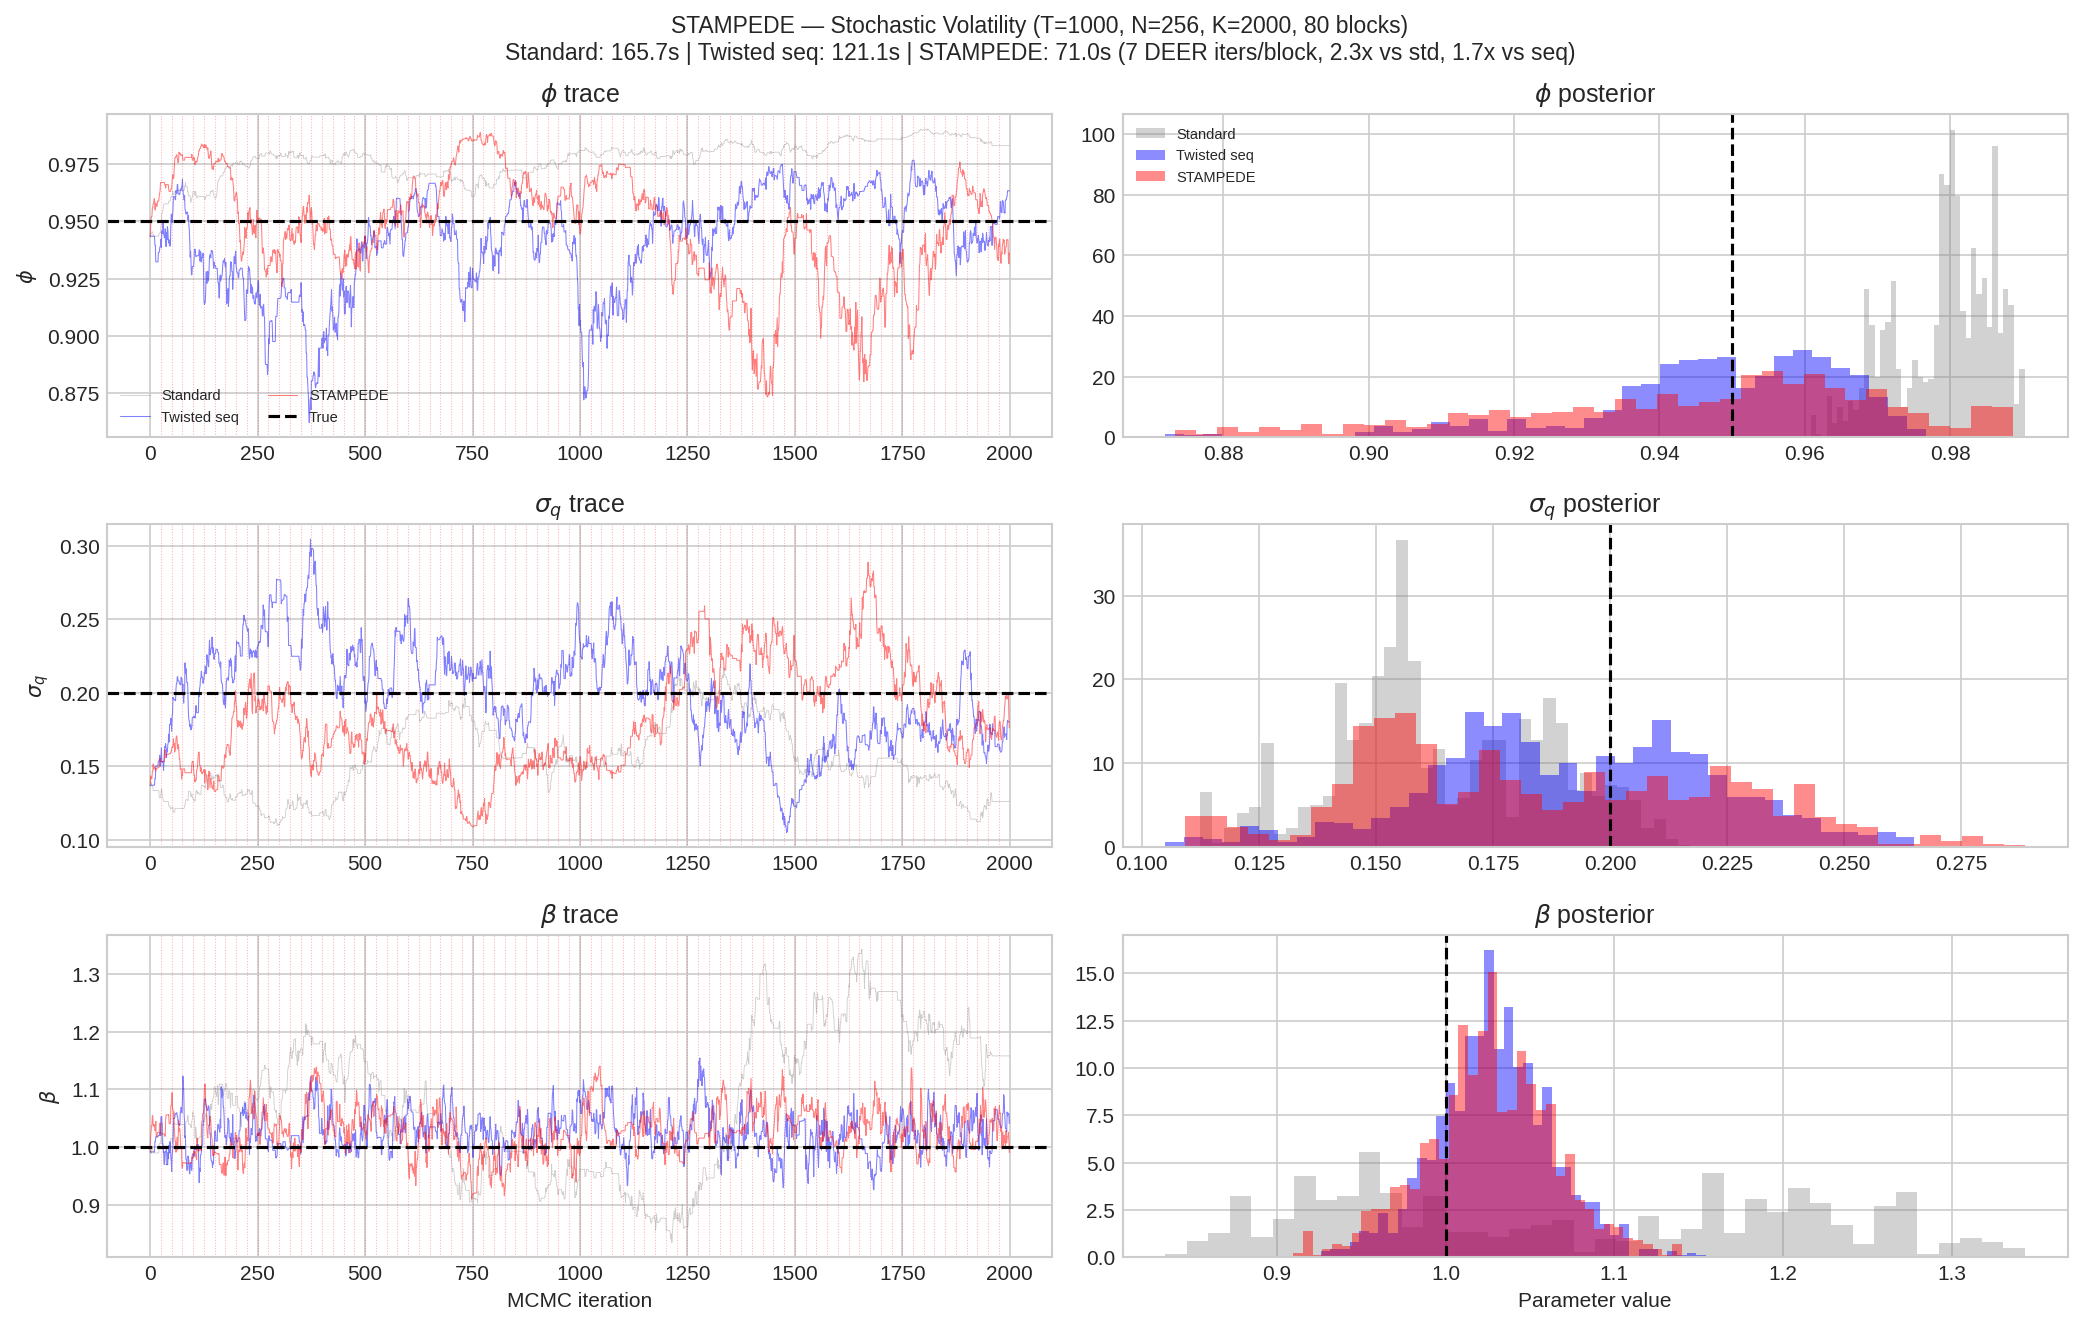
\includegraphics[width=0.92\linewidth]{../stampede_stochvol.png}
    \caption{STAMPEDE on the stochastic volatility model ($T=1000, K=2000$). The grey Standard PMCMC histogram for $\phi$ peaks at $0.98$, far from the true $0.95$; both Twisted seq and STAMPEDE recover the correct posterior, demonstrating that the twisted-DEER smoother is what enables fidelity, while STAMPEDE's outer scan adds a $1.8\times$ wall-clock improvement on top.}
    \label{fig:stampede-stochvol}
\end{figure}

\section{Discussion}
\label{sec:discussion}

\paragraph{When does STAMPEDE win, and by how much?} The empirical pattern is consistent across our experiments. The inner sequence-parallel smoother dominates speedup at large $T$ and modest $D$, scaling from $19\times$ on stochastic volatility to $200\times$ on long LGSSMs. The outer chain-level DEER adds a further $1.5$--$2\times$ on top. STAMPEDE's total speedup over standard bootstrap PMCMC is therefore set by both axes: $2.5$--$2.6\times$ on the moderately-long, moderately-dimensional models we tested, with the gap closing as the per-likelihood cost shrinks at small $T$ or as the latent dimension grows (Section~\ref{sec:exp-pf}).

\paragraph{Where the assumptions break.} Three regimes are challenging. First, when latent dimensions are strongly coupled and large ($D \gg 64$), the full-Jacobian DEER scales as $O(T D^2 N)$ in memory and crosses the cost of the sequential filter; a block-diagonal or rank-structured Jacobian approximation is a natural next step but is not closed under matrix multiplication, so it would need careful design. Second, the chain-level DEER scan grows in iteration count roughly linearly with the block length $K_{\text{blk}}$; the optimum we found ($K_{\text{blk}} \approx 25$) is small relative to the full chain, so the doubly-parallel speedup is bounded by a constant rather than a $\log K$ factor in practice. Third, models with saturating link functions can produce Hessian overflows in DEER on a small subset of chain steps; the quasi-ELK damping resolves this but introduces a hyperparameter $\sigma^2$ that depends on the model's curvature and we tune it by hand.

\paragraph{When NOT to use STAMPEDE.} The bootstrap PF + random-walk MH baseline is hard to beat \emph{per evaluation} on short trajectories because of its $O(T)$ cost with tiny constants. STAMPEDE's compile-time and per-block setup overheads make sense to amortize only when $T$ is at least in the hundreds, the chain length $K$ is at least in the thousands, and the model permits a useful look-ahead twist. Otherwise, the standard baseline can be faster in wall-clock—at the cost of biased posteriors for poorly-mixing models, as quantified by the $4.4\sigma$ $\phi$-bias in stochastic volatility.

\section{Conclusion}
\label{sec:conclusion}

We introduced a sequence-parallel particle smoother that exploits the per-particle factorization of twisted SMC to apply DEER-style associative scans, achieving up to $200\times$ speedup over sequential twisted SMC at bit-equal accuracy. Building on this, we proposed STAMPEDE, a doubly-parallel particle MCMC algorithm whose inner and outer loops are both DEER-accelerated. STAMPEDE delivers $2.5$--$2.6\times$ end-to-end speedups over standard bootstrap PMCMC on linear-Gaussian and stochastic volatility benchmarks while matching or exceeding the posterior fidelity of sequential twisted PMCMC. We see two natural extensions: scaling to large coupled latent dimensions via structured-Jacobian DEER, and combining the twisted-DEER smoother with HMC or NUTS for higher-dimensional parameter spaces.

% \subsection{Style}


% Papers to be submitted to NeurIPS 2026 must be prepared according to the
% instructions presented here. Papers may only be up to {\bf nine} pages long, including figures. \textbf{Papers that exceed the page limit will not be reviewed (or in any other way considered) for presentation at the conference.}
% Additional pages \emph{containing acknowledgments, references, checklist, and optional technical appendices} do not count as content pages. 


% The margins in 2026 are the same as those in previous years.


% Authors are required to use the NeurIPS \LaTeX{} style files obtainable at the NeurIPS website as indicated below. Please make sure you use the current files and not previous versions. Tweaking the style files may be grounds for desk rejection.


% \subsection{Retrieval of style files}


% The style files for NeurIPS and other conference information are available on the website at
% \begin{center}
%   \url{https://neurips.cc}.
% \end{center}
% % The file \verb+neurips_2026.pdf+ contains these instructions and illustrates the various formatting requirements your NeurIPS paper must satisfy.


% The only supported style file for NeurIPS 2026 is \verb+neurips_2026.sty+, rewritten for \LaTeXe{}. \textbf{Previous style files for \LaTeX{} 2.09,  Microsoft Word, and RTF are no longer supported.}


% The \LaTeX{} style file contains three optional arguments: 
% \begin{itemize}
% \item \verb+final+, which creates a camera-ready copy, 
% \item \verb+preprint+, which creates a preprint for submission to, e.g., arXiv, \item \verb+nonatbib+, which will not load the \verb+natbib+ package for you in case of package clash.
% \end{itemize}


% \paragraph{Preprint option}
% If you wish to post a preprint of your work online, e.g., on arXiv, using the NeurIPS style, please use the \verb+preprint+ option. This will create a nonanonymized version of your work with the text ``Preprint. Work in progress.'' in the footer. This version may be distributed as you see fit, as long as you do not say which conference it was submitted to. Please \textbf{do not} use the \verb+final+ option, which should \textbf{only} be used for papers accepted to NeurIPS.


% At submission time, please omit the \verb+final+ and \verb+preprint+ options. This will anonymize your submission and add line numbers to aid review. Please do \emph{not} refer to these line numbers in your paper as they will be removed during generation of camera-ready copies.


% The file \verb+neurips_2026.tex+ may be used as a ``shell'' for writing your paper. All you have to do is replace the author, title, abstract, and text of the paper with your own.


% The formatting instructions contained in these style files are summarized in Sections \ref{gen_inst}, \ref{headings}, and \ref{others} below.


% \section{General formatting instructions}
% \label{gen_inst}


% The text must be confined within a rectangle 5.5~inches (33~picas) wide and
% 9~inches (54~picas) long. The left margin is 1.5~inch (9~picas).  Use 10~point
% type with a vertical spacing (leading) of 11~points.  Times New Roman is the
% preferred typeface throughout, and will be selected for you by default.
% Paragraphs are separated by \nicefrac{1}{2}~line space (5.5 points), with no
% indentation.


% The paper title should be 17~point, initial caps/lower case, bold, centered
% between two horizontal rules. The top rule should be 4~points thick and the
% bottom rule should be 1~point thick. Allow \nicefrac{1}{4}~inch space above and
% below the title to rules. All pages should start at 1~inch (6~picas) from the
% top of the page.


% For the final version, authors' names are set in boldface, and each name is
% centered above the corresponding address. The lead author's name is to be listed
% first (left-most), and the co-authors' names (if different address) are set to
% follow. If there is only one co-author, list both author and co-author side by
% side.


% Please pay special attention to the instructions in Section \ref{others}
% regarding figures, tables, acknowledgments, and references.

% \section{Headings: first level}
% \label{headings}


% All headings should be lower case (except for first word and proper nouns),
% flush left, and bold.


% First-level headings should be in 12-point type.


% \subsection{Headings: second level}


% Second-level headings should be in 10-point type.


% \subsubsection{Headings: third level}


% Third-level headings should be in 10-point type.


% \paragraph{Paragraphs}


% There is also a \verb+\paragraph+ command available, which sets the heading in
% bold, flush left, and inline with the text, with the heading followed by 1\,em
% of space.


% \section{Citations, figures, tables, references}
% \label{others}


% These instructions apply to everyone.


% \subsection{Citations within the text}


% The \verb+natbib+ package will be loaded for you by default.  Citations may be
% author/year or numeric, as long as you maintain internal consistency.  As to the
% format of the references themselves, any style is acceptable as long as it is
% used consistently.


% The documentation for \verb+natbib+ may be found at
% \begin{center}
%   \url{http://mirrors.ctan.org/macros/latex/contrib/natbib/natnotes.pdf}
% \end{center}
% Of note is the command \verb+\citet+, which produces citations appropriate for
% use in inline text.  For example,
% \begin{verbatim}
%    \citet{hasselmo} investigated\dots
% \end{verbatim}
% produces
% \begin{quote}
%   Hasselmo, et al.\ (1995) investigated\dots
% \end{quote}


% If you wish to load the \verb+natbib+ package with options, you may add the
% following before loading the \verb+neurips_2026+ package:
% \begin{verbatim}
%    \PassOptionsToPackage{options}{natbib}
% \end{verbatim}


% If \verb+natbib+ clashes with another package you load, you can add the optional
% argument \verb+nonatbib+ when loading the style file:
% \begin{verbatim}
%    \usepackage[nonatbib]{neurips_2026}
% \end{verbatim}


% As submission is double blind, refer to your own published work in the third
% person. That is, use ``In the previous work of Jones et al.\ [4],'' not ``In our
% previous work [4].'' If you cite your other papers that are not widely available
% (e.g., a journal paper under review), use anonymous author names in the
% citation, e.g., an author of the form ``A.\ Anonymous'' and include a copy of the anonymized paper in the supplementary material.


% \subsection{Footnotes}


% Footnotes should be used sparingly.  If you do require a footnote, indicate
% footnotes with a number\footnote{Sample of the first footnote.} in the
% text. Place the footnotes at the bottom of the page on which they appear.
% Precede the footnote with a horizontal rule of 2~inches (12~picas).


% Note that footnotes are properly typeset \emph{after} punctuation
% marks.\footnote{As in this example.}


% \subsection{Figures}


% \begin{figure}
%   \centering
%   \fbox{\rule[-.5cm]{0cm}{4cm} \rule[-.5cm]{4cm}{0cm}}
%   \caption{Sample figure caption. Explain what the figure shows and add a key take-away message to the caption.}
% \end{figure}


% All artwork must be neat, clean, and legible. Lines should be dark enough for
%  reproduction purposes. The figure number and caption always appear after the
% figure. Place one line space before the figure caption and one line space after
% the figure. The figure caption should be lower case (except for the first word and proper nouns); figures are numbered consecutively.


% You may use color figures.  However, it is best for the figure captions and the
% paper body to be legible if the paper is printed in either black/white or in
% color.


% \subsection{Tables}


% All tables must be centered, neat, clean, and legible.  The table number and
% title always appear before the table.  See Table~\ref{sample-table}.


% Place one line space before the table title, one line space after the
% table title, and one line space after the table. The table title must
% be lower case (except for the first word and proper nouns); tables are
% numbered consecutively.


% Note that publication-quality tables \emph{do not contain vertical rules}. We
% strongly suggest the use of the \verb+booktabs+ package, which allows for
% typesetting high-quality, professional tables:
% \begin{center}
%   \url{https://www.ctan.org/pkg/booktabs}
% \end{center}
% This package was used to typeset Table~\ref{sample-table}.


% \begin{table}
%   \caption{Sample table caption. Explain what the table shows and add a key take-away message to the caption.}
%   \label{sample-table}
%   \centering
%   \begin{tabular}{lll}
%     \toprule
%     \multicolumn{2}{c}{Part}                   \\
%     \cmidrule(r){1-2}
%     Name     & Description     & Size ($\mu$m) \\
%     \midrule
%     Dendrite & Input terminal  & $\approx$100     \\
%     Axon     & Output terminal & $\approx$10      \\
%     Soma     & Cell body       & up to $10^6$  \\
%     \bottomrule
%   \end{tabular}
% \end{table}

% \subsection{Math}
% Note that display math in bare TeX commands will not create correct line numbers for submission. Please use LaTeX (or AMSTeX) commands for unnumbered display math. (You really shouldn't be using \$\$ anyway; see \url{https://tex.stackexchange.com/questions/503/why-is-preferable-to} and \url{https://tex.stackexchange.com/questions/40492/what-are-the-differences-between-align-equation-and-displaymath} for more information.)

% \subsection{Final instructions}

% Do not change any aspects of the formatting parameters in the style files.  In
% particular, do not modify the width or length of the rectangle the text should
% fit into, and do not change font sizes. Please note that pages should be
% numbered.


% \section{Preparing PDF files}


% Please prepare submission files with paper size ``US Letter,'' and not, for
% example, ``A4.''


% Fonts were the main cause of problems in the past years. Your PDF file must only
% contain Type 1 or Embedded TrueType fonts. Here are a few instructions to
% achieve this.


% \begin{itemize}


% \item You should directly generate PDF files using \verb+pdflatex+.


% \item You can check which fonts a PDF files uses.  In Acrobat Reader, select the
%   menu Files$>$Document Properties$>$Fonts and select Show All Fonts. You can
%   also use the program \verb+pdffonts+ which comes with \verb+xpdf+ and is
%   available out-of-the-box on most Linux machines.


% \item \verb+xfig+ ``patterned'' shapes are implemented with bitmap fonts.  Use
%   "solid" shapes instead.


% \item The \verb+\bbold+ package almost always uses bitmap fonts.  You should use
%   the equivalent AMS Fonts:
% \begin{verbatim}
%    \usepackage{amsfonts}
% \end{verbatim}
% followed by, e.g., \verb+\mathbb{R}+, \verb+\mathbb{N}+, or \verb+\mathbb{C}+
% for $\mathbb{R}$, $\mathbb{N}$ or $\mathbb{C}$.  You can also use the following
% workaround for reals, natural and complex:
% \begin{verbatim}
%    \newcommand{\RR}{I\!\!R} %real numbers
%    \newcommand{\Nat}{I\!\!N} %natural numbers
%    \newcommand{\CC}{I\!\!\!\!C} %complex numbers
% \end{verbatim}
% Note that \verb+amsfonts+ is automatically loaded by the \verb+amssymb+ package.


% \end{itemize}


% If your file contains type 3 fonts or non embedded TrueType fonts, we will ask
% you to fix it.


% \subsection{Margins in \LaTeX{}}


% Most of the margin problems come from figures positioned by hand using
% \verb+\special+ or other commands. We suggest using the command
% \verb+\includegraphics+ from the \verb+graphicx+ package. Always specify the
% figure width as a multiple of the line width as in the example below:
% \begin{verbatim}
%    \usepackage[pdftex]{graphicx} ...
%    \includegraphics[width=0.8\linewidth]{myfile.pdf}
% \end{verbatim}
% See Section 4.4 in the graphics bundle documentation
% (\url{http://mirrors.ctan.org/macros/latex/required/graphics/grfguide.pdf})


% A number of width problems arise when \LaTeX{} cannot properly hyphenate a
% line. Please give LaTeX hyphenation hints using the \verb+\-+ command when
% necessary.

% \begin{ack}
% Use unnumbered first level headings for the acknowledgments. All acknowledgments
% go at the end of the paper before the list of references. Moreover, you are required to declare
% funding (financial activities supporting the submitted work) and competing interests (related financial activities outside the submitted work).
% More information about this disclosure can be found at: \url{https://neurips.cc/Conferences/2026/PaperInformation/FundingDisclosure}.


% Do {\bf not} include this section in the anonymized submission, only in the final paper. You can use the \texttt{ack} environment provided in the style file to automatically hide this section in the anonymized submission.
% \end{ack}

% \section*{References}


% References follow the acknowledgments in the camera-ready paper. Use unnumbered first-level heading for
% the references. Any choice of citation style is acceptable as long as you are
% consistent. It is permissible to reduce the font size to \verb+small+ (9 point)
% when listing the references.
% Note that the Reference section does not count towards the page limit.
% \medskip


% {
% \small


% [1] Alexander, J.A.\ \& Mozer, M.C.\ (1995) Template-based algorithms for
% connectionist rule extraction. In G.\ Tesauro, D.S.\ Touretzky and T.K.\ Leen
% (eds.), {\it Advances in Neural Information Processing Systems 7},
% pp.\ 609--616. Cambridge, MA: MIT Press.


% [2] Bower, J.M.\ \& Beeman, D.\ (1995) {\it The Book of GENESIS: Exploring
%   Realistic Neural Models with the GEneral NEural SImulation System.}  New York:
% TELOS/Springer--Verlag.


% [3] Hasselmo, M.E., Schnell, E.\ \& Barkai, E.\ (1995) Dynamics of learning and
% recall at excitatory recurrent synapses and cholinergic modulation in rat
% hippocampal region CA3. {\it Journal of Neuroscience} {\bf 15}(7):5249-5262.
% }


%%%%%%%%%%%%%%%%%%%%%%%%%%%%%%%%%%%%%%%%%%%%%%%%%%%%%%%%%%%%

\appendix

\section{Technical appendices and supplementary material}
Technical appendices with additional results, figures, graphs, and proofs may be submitted with the paper submission before the full submission deadline (see above). You can upload a ZIP file for videos or code, but do not upload a separate PDF file for the appendix. There is no page limit for the technical appendices. 

Note: Think of the appendix as ``optional reading'' for reviewers. The paper must be able to stand alone without the appendix; for example, adding critical experiments that support the main claims to an appendix is inappropriate. 

%%%%%%%%%%%%%%%%%%%%%%%%%%%%%%%%%%%%%%%%%%%%%%%%%%%%%%%%%%%%

\newpage
\section*{NeurIPS Paper Checklist}

%%% BEGIN INSTRUCTIONS %%%
The checklist is designed to encourage best practices for responsible machine learning research, addressing issues of reproducibility, transparency, research ethics, and societal impact. Do not remove the checklist: {\bf The papers not including the checklist will be desk rejected.} The checklist should follow the references and follow the (optional) supplemental material.  The checklist does NOT count towards the page
limit. 

Please read the checklist guidelines carefully for information on how to answer these questions. For each question in the checklist:
\begin{itemize}
    \item You should answer \answerYes{}, \answerNo{}, or \answerNA{}.
    \item \answerNA{} means either that the question is Not Applicable for that particular paper or the relevant information is Not Available.
    \item Please provide a short (1--2 sentence) justification right after your answer (even for \answerNA). 
   % \item {\bf The papers not including the checklist will be desk rejected.}
\end{itemize}

{\bf The checklist answers are an integral part of your paper submission.} They are visible to the reviewers, area chairs, senior area chairs, and ethics reviewers. You will also be asked to include it (after eventual revisions) with the final version of your paper, and its final version will be published with the paper.

The reviewers of your paper will be asked to use the checklist as one of the factors in their evaluation. While \answerYes{} is generally preferable to \answerNo{}, it is perfectly acceptable to answer \answerNo{} provided a proper justification is given (e.g., error bars are not reported because it would be too computationally expensive'' or ``we were unable to find the license for the dataset we used''). In general, answering \answerNo{} or \answerNA{} is not grounds for rejection. While the questions are phrased in a binary way, we acknowledge that the true answer is often more nuanced, so please just use your best judgment and write a justification to elaborate. All supporting evidence can appear either in the main paper or the supplemental material, provided in appendix. If you answer \answerYes{} to a question, in the justification please point to the section(s) where related material for the question can be found.

IMPORTANT, please:
\begin{itemize}
    \item {\bf Delete this instruction block, but keep the section heading ``NeurIPS Paper Checklist"},
    \item  {\bf Keep the checklist subsection headings, questions/answers and guidelines below.}
    \item {\bf Do not modify the questions and only use the provided macros for your answers}.
\end{itemize} 
 

%%% END INSTRUCTIONS %%%


\begin{enumerate}

\item {\bf Claims}
    \item[] Question: Do the main claims made in the abstract and introduction accurately reflect the paper's contributions and scope?
    \item[] Answer: \answerTODO{} % Replace by \answerYes{}, \answerNo{}, or \answerNA{}.
    \item[] Justification: \justificationTODO{}
    \item[] Guidelines:
    \begin{itemize}
        \item The answer \answerNA{} means that the abstract and introduction do not include the claims made in the paper.
        \item The abstract and/or introduction should clearly state the claims made, including the contributions made in the paper and important assumptions and limitations. A \answerNo{} or \answerNA{} answer to this question will not be perceived well by the reviewers. 
        \item The claims made should match theoretical and experimental results, and reflect how much the results can be expected to generalize to other settings. 
        \item It is fine to include aspirational goals as motivation as long as it is clear that these goals are not attained by the paper. 
    \end{itemize}

\item {\bf Limitations}
    \item[] Question: Does the paper discuss the limitations of the work performed by the authors?
    \item[] Answer: \answerTODO{} % Replace by \answerYes{}, \answerNo{}, or \answerNA{}.
    \item[] Justification: \justificationTODO{}
    \item[] Guidelines:
    \begin{itemize}
        \item The answer \answerNA{} means that the paper has no limitation while the answer \answerNo{} means that the paper has limitations, but those are not discussed in the paper. 
        \item The authors are encouraged to create a separate ``Limitations'' section in their paper.
        \item The paper should point out any strong assumptions and how robust the results are to violations of these assumptions (e.g., independence assumptions, noiseless settings, model well-specification, asymptotic approximations only holding locally). The authors should reflect on how these assumptions might be violated in practice and what the implications would be.
        \item The authors should reflect on the scope of the claims made, e.g., if the approach was only tested on a few datasets or with a few runs. In general, empirical results often depend on implicit assumptions, which should be articulated.
        \item The authors should reflect on the factors that influence the performance of the approach. For example, a facial recognition algorithm may perform poorly when image resolution is low or images are taken in low lighting. Or a speech-to-text system might not be used reliably to provide closed captions for online lectures because it fails to handle technical jargon.
        \item The authors should discuss the computational efficiency of the proposed algorithms and how they scale with dataset size.
        \item If applicable, the authors should discuss possible limitations of their approach to address problems of privacy and fairness.
        \item While the authors might fear that complete honesty about limitations might be used by reviewers as grounds for rejection, a worse outcome might be that reviewers discover limitations that aren't acknowledged in the paper. The authors should use their best judgment and recognize that individual actions in favor of transparency play an important role in developing norms that preserve the integrity of the community. Reviewers will be specifically instructed to not penalize honesty concerning limitations.
    \end{itemize}

\item {\bf Theory assumptions and proofs}
    \item[] Question: For each theoretical result, does the paper provide the full set of assumptions and a complete (and correct) proof?
    \item[] Answer: \answerTODO{} % Replace by \answerYes{}, \answerNo{}, or \answerNA{}.
    \item[] Justification: \justificationTODO{}
    \item[] Guidelines:
    \begin{itemize}
        \item The answer \answerNA{} means that the paper does not include theoretical results. 
        \item All the theorems, formulas, and proofs in the paper should be numbered and cross-referenced.
        \item All assumptions should be clearly stated or referenced in the statement of any theorems.
        \item The proofs can either appear in the main paper or the supplemental material, but if they appear in the supplemental material, the authors are encouraged to provide a short proof sketch to provide intuition. 
        \item Inversely, any informal proof provided in the core of the paper should be complemented by formal proofs provided in appendix or supplemental material.
        \item Theorems and Lemmas that the proof relies upon should be properly referenced. 
    \end{itemize}

    \item {\bf Experimental result reproducibility}
    \item[] Question: Does the paper fully disclose all the information needed to reproduce the main experimental results of the paper to the extent that it affects the main claims and/or conclusions of the paper (regardless of whether the code and data are provided or not)?
    \item[] Answer: \answerTODO{} % Replace by \answerYes{}, \answerNo{}, or \answerNA{}.
    \item[] Justification: \justificationTODO{}
    \item[] Guidelines:
    \begin{itemize}
        \item The answer \answerNA{} means that the paper does not include experiments.
        \item If the paper includes experiments, a \answerNo{} answer to this question will not be perceived well by the reviewers: Making the paper reproducible is important, regardless of whether the code and data are provided or not.
        \item If the contribution is a dataset and\slash or model, the authors should describe the steps taken to make their results reproducible or verifiable. 
        \item Depending on the contribution, reproducibility can be accomplished in various ways. For example, if the contribution is a novel architecture, describing the architecture fully might suffice, or if the contribution is a specific model and empirical evaluation, it may be necessary to either make it possible for others to replicate the model with the same dataset, or provide access to the model. In general. releasing code and data is often one good way to accomplish this, but reproducibility can also be provided via detailed instructions for how to replicate the results, access to a hosted model (e.g., in the case of a large language model), releasing of a model checkpoint, or other means that are appropriate to the research performed.
        \item While NeurIPS does not require releasing code, the conference does require all submissions to provide some reasonable avenue for reproducibility, which may depend on the nature of the contribution. For example
        \begin{enumerate}
            \item If the contribution is primarily a new algorithm, the paper should make it clear how to reproduce that algorithm.
            \item If the contribution is primarily a new model architecture, the paper should describe the architecture clearly and fully.
            \item If the contribution is a new model (e.g., a large language model), then there should either be a way to access this model for reproducing the results or a way to reproduce the model (e.g., with an open-source dataset or instructions for how to construct the dataset).
            \item We recognize that reproducibility may be tricky in some cases, in which case authors are welcome to describe the particular way they provide for reproducibility. In the case of closed-source models, it may be that access to the model is limited in some way (e.g., to registered users), but it should be possible for other researchers to have some path to reproducing or verifying the results.
        \end{enumerate}
    \end{itemize}


\item {\bf Open access to data and code}
    \item[] Question: Does the paper provide open access to the data and code, with sufficient instructions to faithfully reproduce the main experimental results, as described in supplemental material?
    \item[] Answer: \answerTODO{} % Replace by \answerYes{}, \answerNo{}, or \answerNA{}.
    \item[] Justification: \justificationTODO{}
    \item[] Guidelines:
    \begin{itemize}
        \item The answer \answerNA{} means that paper does not include experiments requiring code.
        \item Please see the NeurIPS code and data submission guidelines (\url{https://neurips.cc/public/guides/CodeSubmissionPolicy}) for more details.
        \item While we encourage the release of code and data, we understand that this might not be possible, so \answerNo{} is an acceptable answer. Papers cannot be rejected simply for not including code, unless this is central to the contribution (e.g., for a new open-source benchmark).
        \item The instructions should contain the exact command and environment needed to run to reproduce the results. See the NeurIPS code and data submission guidelines (\url{https://neurips.cc/public/guides/CodeSubmissionPolicy}) for more details.
        \item The authors should provide instructions on data access and preparation, including how to access the raw data, preprocessed data, intermediate data, and generated data, etc.
        \item The authors should provide scripts to reproduce all experimental results for the new proposed method and baselines. If only a subset of experiments are reproducible, they should state which ones are omitted from the script and why.
        \item At submission time, to preserve anonymity, the authors should release anonymized versions (if applicable).
        \item Providing as much information as possible in supplemental material (appended to the paper) is recommended, but including URLs to data and code is permitted.
    \end{itemize}


\item {\bf Experimental setting/details}
    \item[] Question: Does the paper specify all the training and test details (e.g., data splits, hyperparameters, how they were chosen, type of optimizer) necessary to understand the results?
    \item[] Answer: \answerTODO{} % Replace by \answerYes{}, \answerNo{}, or \answerNA{}.
    \item[] Justification: \justificationTODO{}
    \item[] Guidelines:
    \begin{itemize}
        \item The answer \answerNA{} means that the paper does not include experiments.
        \item The experimental setting should be presented in the core of the paper to a level of detail that is necessary to appreciate the results and make sense of them.
        \item The full details can be provided either with the code, in appendix, or as supplemental material.
    \end{itemize}

\item {\bf Experiment statistical significance}
    \item[] Question: Does the paper report error bars suitably and correctly defined or other appropriate information about the statistical significance of the experiments?
    \item[] Answer: \answerTODO{} % Replace by \answerYes{}, \answerNo{}, or \answerNA{}.
    \item[] Justification: \justificationTODO{}
    \item[] Guidelines:
    \begin{itemize}
        \item The answer \answerNA{} means that the paper does not include experiments.
        \item The authors should answer \answerYes{} if the results are accompanied by error bars, confidence intervals, or statistical significance tests, at least for the experiments that support the main claims of the paper.
        \item The factors of variability that the error bars are capturing should be clearly stated (for example, train/test split, initialization, random drawing of some parameter, or overall run with given experimental conditions).
        \item The method for calculating the error bars should be explained (closed form formula, call to a library function, bootstrap, etc.)
        \item The assumptions made should be given (e.g., Normally distributed errors).
        \item It should be clear whether the error bar is the standard deviation or the standard error of the mean.
        \item It is OK to report 1-sigma error bars, but one should state it. The authors should preferably report a 2-sigma error bar than state that they have a 96\% CI, if the hypothesis of Normality of errors is not verified.
        \item For asymmetric distributions, the authors should be careful not to show in tables or figures symmetric error bars that would yield results that are out of range (e.g., negative error rates).
        \item If error bars are reported in tables or plots, the authors should explain in the text how they were calculated and reference the corresponding figures or tables in the text.
    \end{itemize}

\item {\bf Experiments compute resources}
    \item[] Question: For each experiment, does the paper provide sufficient information on the computer resources (type of compute workers, memory, time of execution) needed to reproduce the experiments?
    \item[] Answer: \answerTODO{} % Replace by \answerYes{}, \answerNo{}, or \answerNA{}.
    \item[] Justification: \justificationTODO{}
    \item[] Guidelines:
    \begin{itemize}
        \item The answer \answerNA{} means that the paper does not include experiments.
        \item The paper should indicate the type of compute workers CPU or GPU, internal cluster, or cloud provider, including relevant memory and storage.
        \item The paper should provide the amount of compute required for each of the individual experimental runs as well as estimate the total compute. 
        \item The paper should disclose whether the full research project required more compute than the experiments reported in the paper (e.g., preliminary or failed experiments that didn't make it into the paper). 
    \end{itemize}
    
\item {\bf Code of ethics}
    \item[] Question: Does the research conducted in the paper conform, in every respect, with the NeurIPS Code of Ethics \url{https://neurips.cc/public/EthicsGuidelines}?
    \item[] Answer: \answerTODO{} % Replace by \answerYes{}, \answerNo{}, or \answerNA{}.
    \item[] Justification: \justificationTODO{}
    \item[] Guidelines:
    \begin{itemize}
        \item The answer \answerNA{} means that the authors have not reviewed the NeurIPS Code of Ethics.
        \item If the authors answer \answerNo, they should explain the special circumstances that require a deviation from the Code of Ethics.
        \item The authors should make sure to preserve anonymity (e.g., if there is a special consideration due to laws or regulations in their jurisdiction).
    \end{itemize}


\item {\bf Broader impacts}
    \item[] Question: Does the paper discuss both potential positive societal impacts and negative societal impacts of the work performed?
    \item[] Answer: \answerTODO{} % Replace by \answerYes{}, \answerNo{}, or \answerNA{}.
    \item[] Justification: \justificationTODO{}
    \item[] Guidelines:
    \begin{itemize}
        \item The answer \answerNA{} means that there is no societal impact of the work performed.
        \item If the authors answer \answerNA{} or \answerNo, they should explain why their work has no societal impact or why the paper does not address societal impact.
        \item Examples of negative societal impacts include potential malicious or unintended uses (e.g., disinformation, generating fake profiles, surveillance), fairness considerations (e.g., deployment of technologies that could make decisions that unfairly impact specific groups), privacy considerations, and security considerations.
        \item The conference expects that many papers will be foundational research and not tied to particular applications, let alone deployments. However, if there is a direct path to any negative applications, the authors should point it out. For example, it is legitimate to point out that an improvement in the quality of generative models could be used to generate Deepfakes for disinformation. On the other hand, it is not needed to point out that a generic algorithm for optimizing neural networks could enable people to train models that generate Deepfakes faster.
        \item The authors should consider possible harms that could arise when the technology is being used as intended and functioning correctly, harms that could arise when the technology is being used as intended but gives incorrect results, and harms following from (intentional or unintentional) misuse of the technology.
        \item If there are negative societal impacts, the authors could also discuss possible mitigation strategies (e.g., gated release of models, providing defenses in addition to attacks, mechanisms for monitoring misuse, mechanisms to monitor how a system learns from feedback over time, improving the efficiency and accessibility of ML).
    \end{itemize}
    
\item {\bf Safeguards}
    \item[] Question: Does the paper describe safeguards that have been put in place for responsible release of data or models that have a high risk for misuse (e.g., pre-trained language models, image generators, or scraped datasets)?
    \item[] Answer: \answerTODO{} % Replace by \answerYes{}, \answerNo{}, or \answerNA{}.
    \item[] Justification: \justificationTODO{}
    \item[] Guidelines:
    \begin{itemize}
        \item The answer \answerNA{} means that the paper poses no such risks.
        \item Released models that have a high risk for misuse or dual-use should be released with necessary safeguards to allow for controlled use of the model, for example by requiring that users adhere to usage guidelines or restrictions to access the model or implementing safety filters. 
        \item Datasets that have been scraped from the Internet could pose safety risks. The authors should describe how they avoided releasing unsafe images.
        \item We recognize that providing effective safeguards is challenging, and many papers do not require this, but we encourage authors to take this into account and make a best faith effort.
    \end{itemize}

\item {\bf Licenses for existing assets}
    \item[] Question: Are the creators or original owners of assets (e.g., code, data, models), used in the paper, properly credited and are the license and terms of use explicitly mentioned and properly respected?
    \item[] Answer: \answerTODO{} % Replace by \answerYes{}, \answerNo{}, or \answerNA{}.
    \item[] Justification: \justificationTODO{}
    \item[] Guidelines:
    \begin{itemize}
        \item The answer \answerNA{} means that the paper does not use existing assets.
        \item The authors should cite the original paper that produced the code package or dataset.
        \item The authors should state which version of the asset is used and, if possible, include a URL.
        \item The name of the license (e.g., CC-BY 4.0) should be included for each asset.
        \item For scraped data from a particular source (e.g., website), the copyright and terms of service of that source should be provided.
        \item If assets are released, the license, copyright information, and terms of use in the package should be provided. For popular datasets, \url{paperswithcode.com/datasets} has curated licenses for some datasets. Their licensing guide can help determine the license of a dataset.
        \item For existing datasets that are re-packaged, both the original license and the license of the derived asset (if it has changed) should be provided.
        \item If this information is not available online, the authors are encouraged to reach out to the asset's creators.
    \end{itemize}

\item {\bf New assets}
    \item[] Question: Are new assets introduced in the paper well documented and is the documentation provided alongside the assets?
    \item[] Answer: \answerTODO{} % Replace by \answerYes{}, \answerNo{}, or \answerNA{}.
    \item[] Justification: \justificationTODO{}
    \item[] Guidelines:
    \begin{itemize}
        \item The answer \answerNA{} means that the paper does not release new assets.
        \item Researchers should communicate the details of the dataset\slash code\slash model as part of their submissions via structured templates. This includes details about training, license, limitations, etc. 
        \item The paper should discuss whether and how consent was obtained from people whose asset is used.
        \item At submission time, remember to anonymize your assets (if applicable). You can either create an anonymized URL or include an anonymized zip file.
    \end{itemize}

\item {\bf Crowdsourcing and research with human subjects}
    \item[] Question: For crowdsourcing experiments and research with human subjects, does the paper include the full text of instructions given to participants and screenshots, if applicable, as well as details about compensation (if any)? 
    \item[] Answer: \answerTODO{} % Replace by \answerYes{}, \answerNo{}, or \answerNA{}.
    \item[] Justification: \justificationTODO{}
    \item[] Guidelines:
    \begin{itemize}
        \item The answer \answerNA{} means that the paper does not involve crowdsourcing nor research with human subjects.
        \item Including this information in the supplemental material is fine, but if the main contribution of the paper involves human subjects, then as much detail as possible should be included in the main paper. 
        \item According to the NeurIPS Code of Ethics, workers involved in data collection, curation, or other labor should be paid at least the minimum wage in the country of the data collector. 
    \end{itemize}

\item {\bf Institutional review board (IRB) approvals or equivalent for research with human subjects}
    \item[] Question: Does the paper describe potential risks incurred by study participants, whether such risks were disclosed to the subjects, and whether Institutional Review Board (IRB) approvals (or an equivalent approval/review based on the requirements of your country or institution) were obtained?
    \item[] Answer: \answerTODO{} % Replace by \answerYes{}, \answerNo{}, or \answerNA{}.
    \item[] Justification: \justificationTODO{}
    \item[] Guidelines:
    \begin{itemize}
        \item The answer \answerNA{} means that the paper does not involve crowdsourcing nor research with human subjects.
        \item Depending on the country in which research is conducted, IRB approval (or equivalent) may be required for any human subjects research. If you obtained IRB approval, you should clearly state this in the paper. 
        \item We recognize that the procedures for this may vary significantly between institutions and locations, and we expect authors to adhere to the NeurIPS Code of Ethics and the guidelines for their institution. 
        \item For initial submissions, do not include any information that would break anonymity (if applicable), such as the institution conducting the review.
    \end{itemize}

\item {\bf Declaration of LLM usage}
    \item[] Question: Does the paper describe the usage of LLMs if it is an important, original, or non-standard component of the core methods in this research? Note that if the LLM is used only for writing, editing, or formatting purposes and does \emph{not} impact the core methodology, scientific rigor, or originality of the research, declaration is not required.
    %this research? 
    \item[] Answer: \answerTODO{} % Replace by \answerYes{}, \answerNo{}, or \answerNA{}.
    \item[] Justification: \justificationTODO{}
    \item[] Guidelines:
    \begin{itemize}
        \item The answer \answerNA{} means that the core method development in this research does not involve LLMs as any important, original, or non-standard components.
        \item Please refer to our LLM policy in the NeurIPS handbook for what should or should not be described.
    \end{itemize}

\end{enumerate}


\end{document}